\documentclass[11pt,a4paper]{article}
\usepackage[UTF8]{ctex}
\usepackage{amsmath,amssymb,bm}
\usepackage{graphicx}
\usepackage{booktabs,multirow,array,longtable}
\usepackage{geometry}
\usepackage{caption}
\usepackage{multicol}
\usepackage{enumitem}
\usepackage{algorithm,algpseudocode}
\usepackage{amsthm}
\usepackage{float}
\usepackage[hidelinks]{hyperref}
\geometry{left=2.4cm,right=2.4cm,top=2.4cm,bottom=2.2cm}
\captionsetup{font=small,labelsep=quad}
\newtheorem{proposition}{命题}
\newtheorem{definition}{定义}
\newcommand{\E}{\mathbb{E}}
\newcommand{\R}{\mathbb{R}}
% 长标识符（\textbackslash section、ax.set_title(...)、“deliverable”: true）
% 在 \texttt 里缺少断点，容易冲出页边。下面三项一起放宽断行：
% emergencystretch 允许在紧急情况下拉伸词间空隙，tolerance 提高容忍度，
% hbadness 关掉“欠满”报告（本文长表格多，欠满提示无信息量）。
\setlength{\emergencystretch}{5em}
\tolerance=3000
\hbadness=10000
\newcommand{\code}[1]{\texttt{#1}}
\title{\vspace{-1.2cm}\textbf{一个会拒绝的系统}\\[2pt]
\large LLM 辅助科研中验证护栏的演进、实证与自我否证\\[2pt]
\normalsize ——一份系统性回顾（R1--R125）}
\author{KuoTzuyang\\[2pt]
\small 塔里木大学\quad 数据科学与大数据（NIIT）\quad 2026 级 4 班}
\date{2026 年 11 月 12 日}
\begin{document}
\maketitle
\vspace{-0.6cm}

%==================================================== 摘要
\begin{center}\rule{0.95\textwidth}{0.4pt}\end{center}
\begin{center}\textbf{摘\quad 要}\end{center}

大语言模型能写出通顺的报告，也会编造数字。要求模型“仔细一点”在截止日期前不可依赖，
因此本文采取另一条路线：在模型旁边建一个\textbf{会拒绝}的程序——它负责计算、记录溯源，
并拒绝为无法溯源的数字或无法被攻破的论断签署通过。

本文不是把一个工具的功能罗列一遍，而是\textbf{系统回顾它如何长成现在这样}：
从能力层（\code{mmkit.py}，当前 23 个子命令）的建立，到门禁系统从 23 项扩到
\textbf{35 项}（硬门 12、软门 23）的每一轮扩张；从“检查项靠记忆列”到
“板块数必须等于论文的 \code{\textbackslash section} 数”这一约束的落地；
以及四次\textbf{由该工具自己抓出来的自欺}。第四次与前三次不同：前三次由用户指令或外部评审触发，第四次是系统自己数出来的——它数出 35 项门禁里只有 4 项同时具备构造缺陷与变异敏感，覆盖率 11.4\%。这个把自己判负的结果，直接导致本文从“数门”改为“分层”。每一次扩张都由一个具体的失败触发，
我们把触发事件、修补方式与修补后的实测数字一并记录。

本文的第二项贡献是把 35 项门禁按它们检查的\emph{对象}重分为四层——值、推导、过程、以及元层的“过程不发散”——并论证内容层到三层为止有理由（存在不可能性结果），而元层不是“更上一层的内容”，是另一个坐标轴。本文的核心方法论贡献是一条举证标准：\textbf{报告“拦住了 $N/M$”不构成任何证据}。
样本可以被作者挑选、期望可以被作者设定、判定可以被作者实现——前两条无法在一个作者、
一个语料的前提下根除，第三条必须根除。可接受的证据只有一种：
\textbf{构造一个缺陷样本，调用真实的护栏，然后把护栏改坏，确认样本随之从“拦住”变成“漏检”}。
我们实现并运行了这一变异测试，当前结果为\textbf{假测试 0/4}。

本文同时记录\textbf{尚未做到的事}，因为一份只报告成功的回顾没有信息量：
35 项门禁中只有 4 项具备“构造缺陷 + 变异覆盖”，其余 31 项是判据实现而非经过检验的测试；
零 baseline 对比；A/B 对照实验仅 $n=1$；24 张图的人工逐张核对在规则写出后\textbf{并未执行}。
数字类别分布实测表明：23 篇报告共 9\,337 个数字按来源分四类，\textbf{计算值 47.3\%}、配置值 27.1\%、结构性 17.6\%、时间标签 8.0\%。后三类合计 52.7\% 可由知识源与数据结构解释，\textbf{只有 47.3\% 必须来自一次实际计算}——这是“需要计算谱系判据”而非“需要更强知识库”的量化依据。若把后三类也一并要求出处，近半数告警会是误报。

最后，本文用两个真实产出检验这条链路：一个 16 页的智算集群规划论文（由该链路生产），
以及一个向量数据库实现的 14 个缺陷（该链路作为审计方，以“通过者的测试”当探针）。

\textbf{关键词}：验证护栏；数字溯源；变异测试；失败关闭；LLM 事实性；自我否证

\newpage
% 目录压到一页：收紧条目间距，避免附录条目单独溢出成一张近乎空白的纸
{\footnotesize
\setlength{\parskip}{0pt}
\makeatletter
\renewcommand{\l@section}{\@dottedtocline{1}{0em}{1.7em}}
\renewcommand{\l@subsection}{\@dottedtocline{2}{1.7em}{2.4em}}
\makeatother
\renewcommand{\contentsname}{目\quad 录}
\begin{multicols}{2}
\tableofcontents
\end{multicols}}
\newpage

%==================================================== 1
\section{引言：为什么需要一个会拒绝的程序}
\noindent\emph{本文的写法遵循系统综述的报告规范\cite{ref17,ref18}：每一节都给出触发事件、修补方式与修补后的实测数字，并把\emph{没做到的事}单列一节。}

现有的事实性评测把问题定义为“这句话能否被知识源支持”\cite{ref13,ref14}，这一定义不覆盖计算得到的数值。

\subsection{问题}
大语言模型写出的报告有一个稳定的失效模式：\textbf{叙述会被悄悄调整到与它并未真正计算过的数字相匹配}。
这不是模型“不够仔细”，而是在生成式框架下，文字与计算之间没有强制通路。
把要求写进提示词（“所有数字必须有出处”）能改善表面表现，但在截止日期、
长文档、多轮修改的条件下不可依赖——因为\textbf{没有任何机制会在违反时阻止交付}。

\subsection{本文的立场}
我们把责任从“作者的用心”转移到“一个可以说不的程序”上。具体做法是在模型旁边设三层：

\begin{enumerate}[leftmargin=1.6em,itemsep=2pt]
\item \textbf{能力层}：只做计算与验证，从不写散文。当前 23 个子命令，覆盖描述统计、
  预测、优化、评价、聚类、图论、常微分方程、量纲分析等。
\item \textbf{决策层}：即 LLM 本身，读题、定方法、组织论证、写正文。
\item \textbf{门禁层}：35 道检查，其中 12 道为硬门。硬门任一失败、或警告不为零，
  则该稿不算完成。门禁\textbf{失败关闭}：数字没有出处就不通过；检查无法执行时
  报“不适用”而不是报“通过”。
\end{enumerate}

三层分离是刻意的。能力层不写散文，决策层不算数——这阻断了“叙述迁就数字”的最短路径。

\subsection{本文不做什么}
\textbf{本文不是一个工具的说明书。}罗列命令与参数对读者没有价值，那些在
\code{schema.json} 里可以自动生成。本文要回答的是三个更难的问题：
\begin{enumerate}[leftmargin=1.6em,itemsep=2pt]
\item 这套护栏是\textbf{怎么演化成现在这样}的？每一次扩张由什么触发？
\item 我们凭什么相信某道门\textbf{真的有效}，而不是恰好没有缺陷通过？
\item 哪些门\textbf{其实没被检验过}？——这一节的长度，是本文可信度的主要来源。
\end{enumerate}

%==================================================== 2
\section{系统总览与演进分期}

\subsection{三个组件的分工与成本}
表 \ref{tab:layers} 给出三个组件各自的实测成本。数据来自能力层 30 次重复自检与（图~\ref{fig:layers}）（图~\ref{fig:arch}）
一整篇交付论文的端到端计时。

\begin{figure}[tbp]\centering
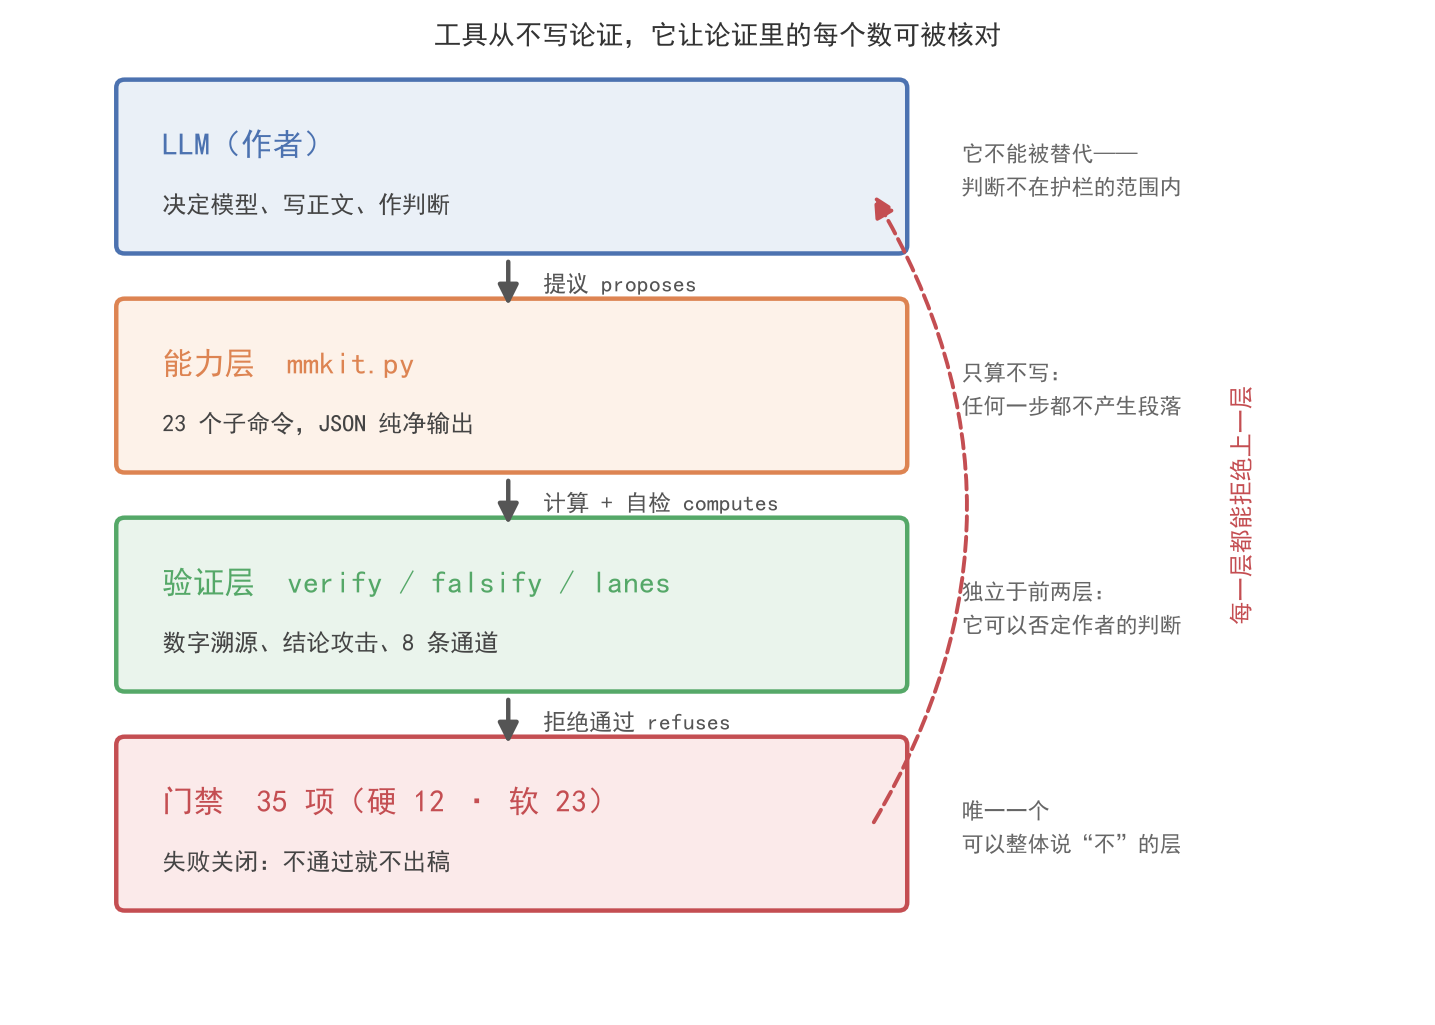
\includegraphics[width=0.86\textwidth]{figs/figK_arch.png}
\caption{四层分工。模型是作者，工具从不写论证；每一层都可以拒绝上一层——门禁可以整体说“不”，验证层可以否定作者的判断，能力层可以拒绝执行不可算的步骤。虚线是这条拒绝链。}
\label{fig:arch}
\end{figure}

\begin{table}[tbp]\centering\small
\caption{三个组件的实测成本（来源：能力层 30 次重复自检 + 端到端计时）}\label{tab:layers}

\setlength{\tabcolsep}{4pt}
\begin{tabular}{llrr}
\toprule
层 & 内容 & 成本 & 占一篇论文墙钟 \\
\midrule
能力层 & 7 项能力 / 93 项自检 & 1.191 s & 0.11\% \\
验证与编译 & 4 个验证脚本 + 2 遍 \LaTeX & 7.97 s & 0.71\% \\
机器侧合计 & 以上全部 & \textbf{9.16 s} & \textbf{0.82\%} \\
决策层 & LLM 读题、定方法、写正文 & 1\,114.8 s & 99.18\% \\
\midrule
合计 & 一篇交付论文 & 1\,124 s & 100\% \\
\bottomrule
\end{tabular}
\end{table}
四层分工在早期版本（插件论文第 6 页）就已确定：LLM 决定模型并写正文，
插件负责计算，验证层独立于二者、并可以拒绝上一层。
\textbf{本文不复印那张截图}——它与本节文字重复，且会带进原稿的图号与表号。

这张表本身是一个结论：\textbf{机器侧只占 0.82\% 的墙钟}。因此“护栏拖慢生产”不成立，

\begin{figure}[tbp]\centering
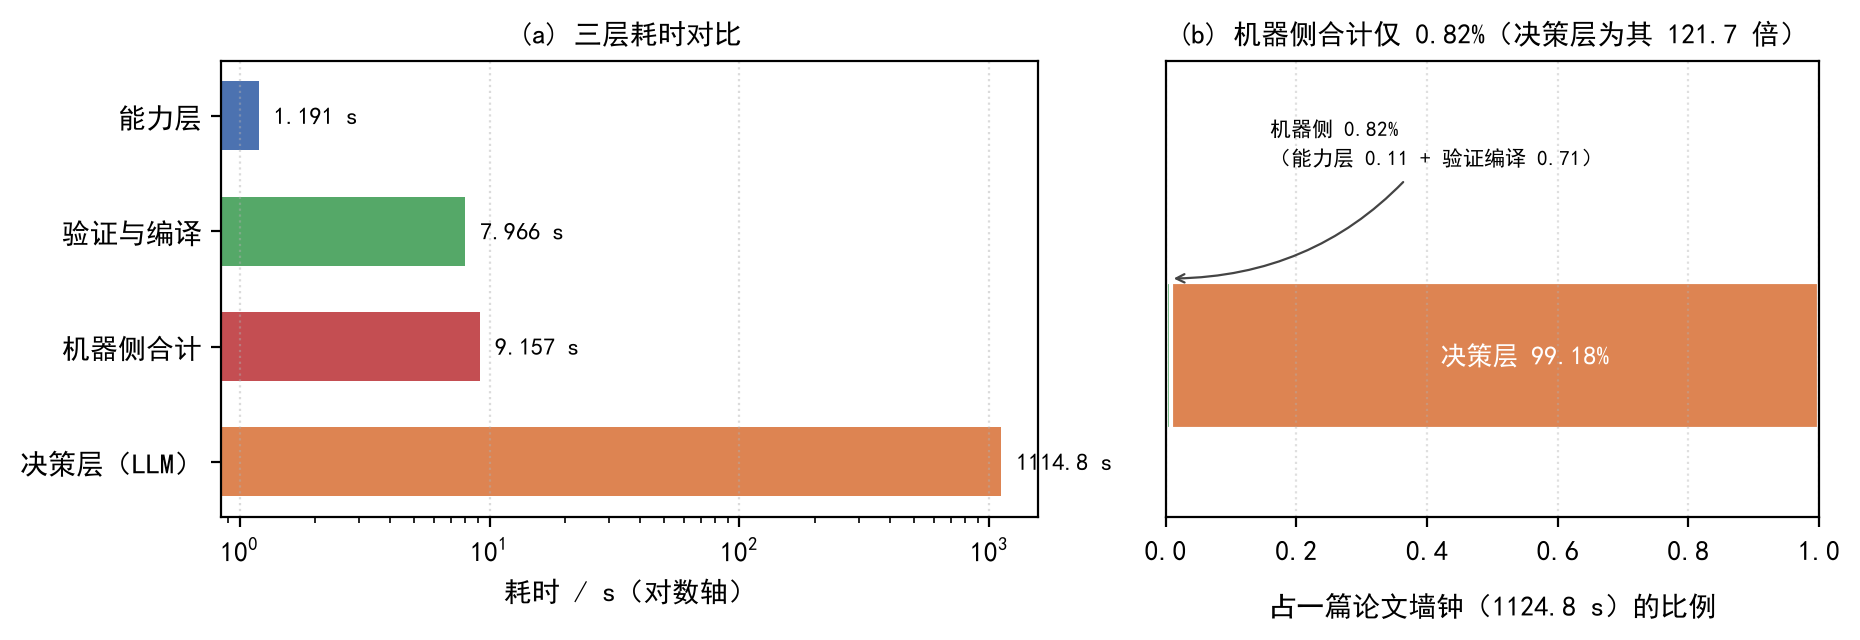
\includegraphics[width=0.92\textwidth]{figs/figA_layers.png}
\caption{三层耗时与占比。(a) 对数轴上决策层比机器侧高两个数量级；(b) 堆叠条显示机器侧合计仅占一篇论文墙钟的 0.82\%。这张图是「护栏拖慢生产」这一说法不成立的直接依据。}\label{fig:layers}
\end{figure}

不装护栏的理由不能是时间。

\subsection{能力之间的效率差 52 倍}
同样重要的是：能力之间并不等价。表 \ref{tab:capcost} 按“每秒自检数”排序，（图~\ref{fig:capcost}）
最高与最低相差\textbf{52 倍}（398.4 对 7.6）。这直接否证了“先用最快的”这一朴素调度规则——

\begin{figure}[tbp]\centering
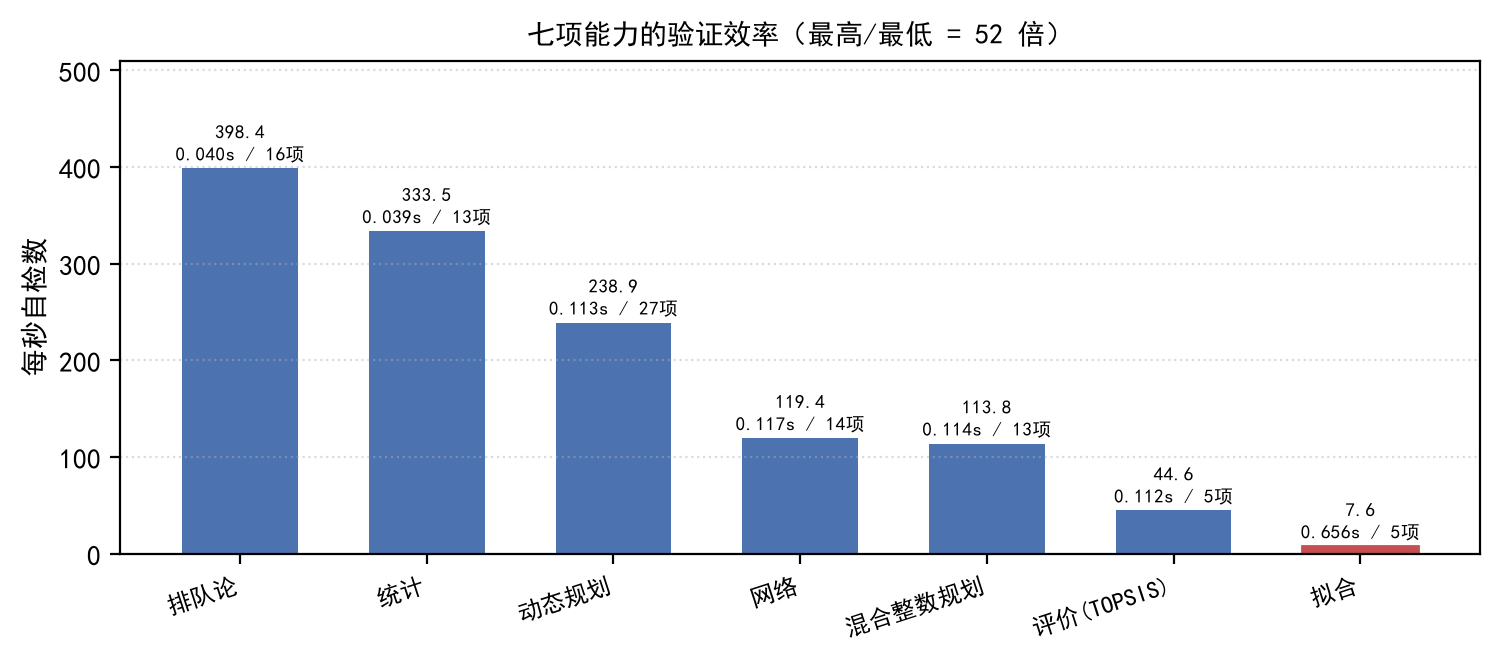
\includegraphics[width=0.92\textwidth]{figs/figB_capcost.png}
\caption{七项能力的验证效率。拟合类每次自检 0.656\,s，排队论 0.040\,s，按耗时差 16 倍；换算成每秒自检数则差 52 倍。这否证了「先跑最快的」这一朴素调度规则。}\label{fig:capcost}
\end{figure}

在需要覆盖某个数学结构时，慢的那项可能无可替代。



\begin{table}[tbp]\centering\small
\caption{各能力的自检成本（每项 30 次重复，全部通过）}\label{tab:capcost}
\setlength{\tabcolsep}{4pt}
\begin{tabular}{lrrrr}
\toprule
能力 & 自检数 & 均耗时 (s) & 标准差 (s) & 每秒自检数\\
\midrule
排队论 & 16 & 0.040 & 0.006 & 398.4\\
统计 & 13 & 0.039 & 0.004 & 333.5\\
动态规划 & 27 & 0.113 & 0.005 & 238.9\\
网络 & 14 & 0.117 & 0.006 & 119.4\\
混合整数规划 & 13 & 0.114 & 0.005 & 113.8\\
评价（TOPSIS） & 5 & 0.112 & 0.006 & 44.6\\
拟合 & 5 & 0.656 & 0.032 & \textbf{7.6}\\
\midrule
合计 & 93 & 1.191 & — & 78.1\\
\bottomrule
\end{tabular}
\end{table}

\subsection{演进分期}

\begin{figure}[tbp]\centering
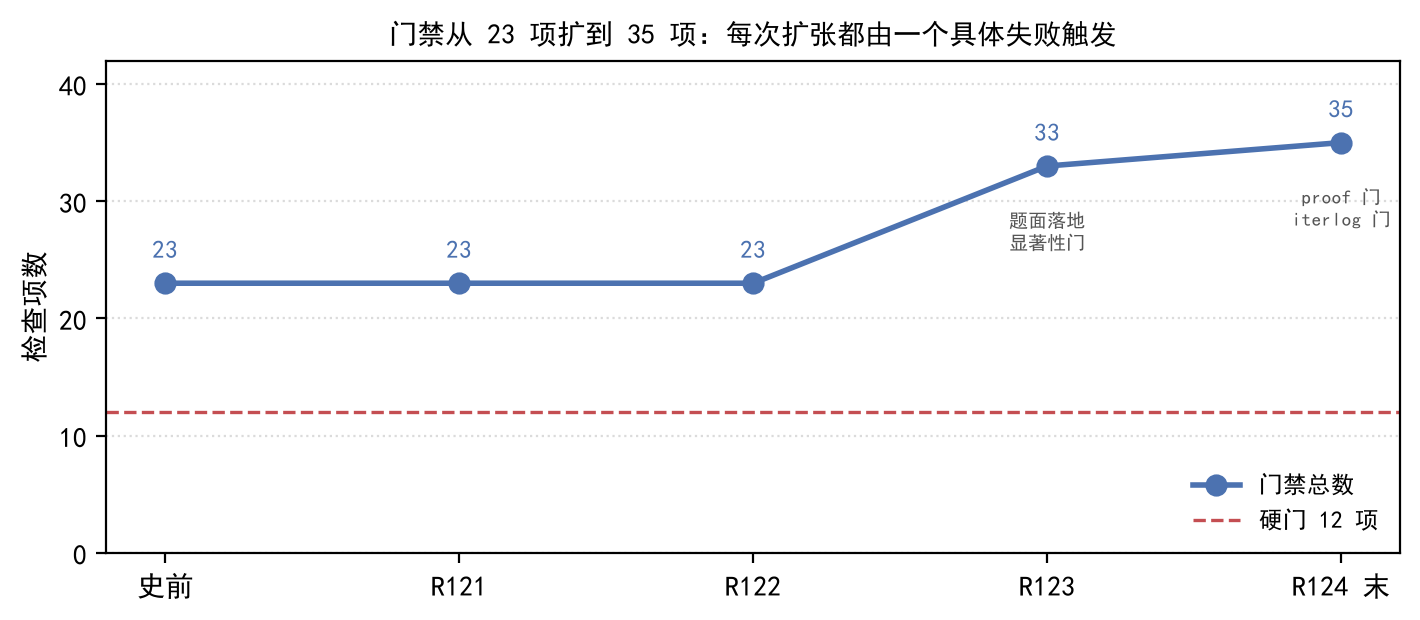
\includegraphics[width=0.92\textwidth]{figs/figD_gategrowth.png}
\caption{门禁从 23 项扩到 35 项的过程。每一次跳跃都对应 §\ref{tab:phases} 中的一个触发事件，而不是计划性扩张；硬门始终维持 12 项。}\label{fig:gategrowth}
\end{figure}

\begin{figure}[tbp]\centering
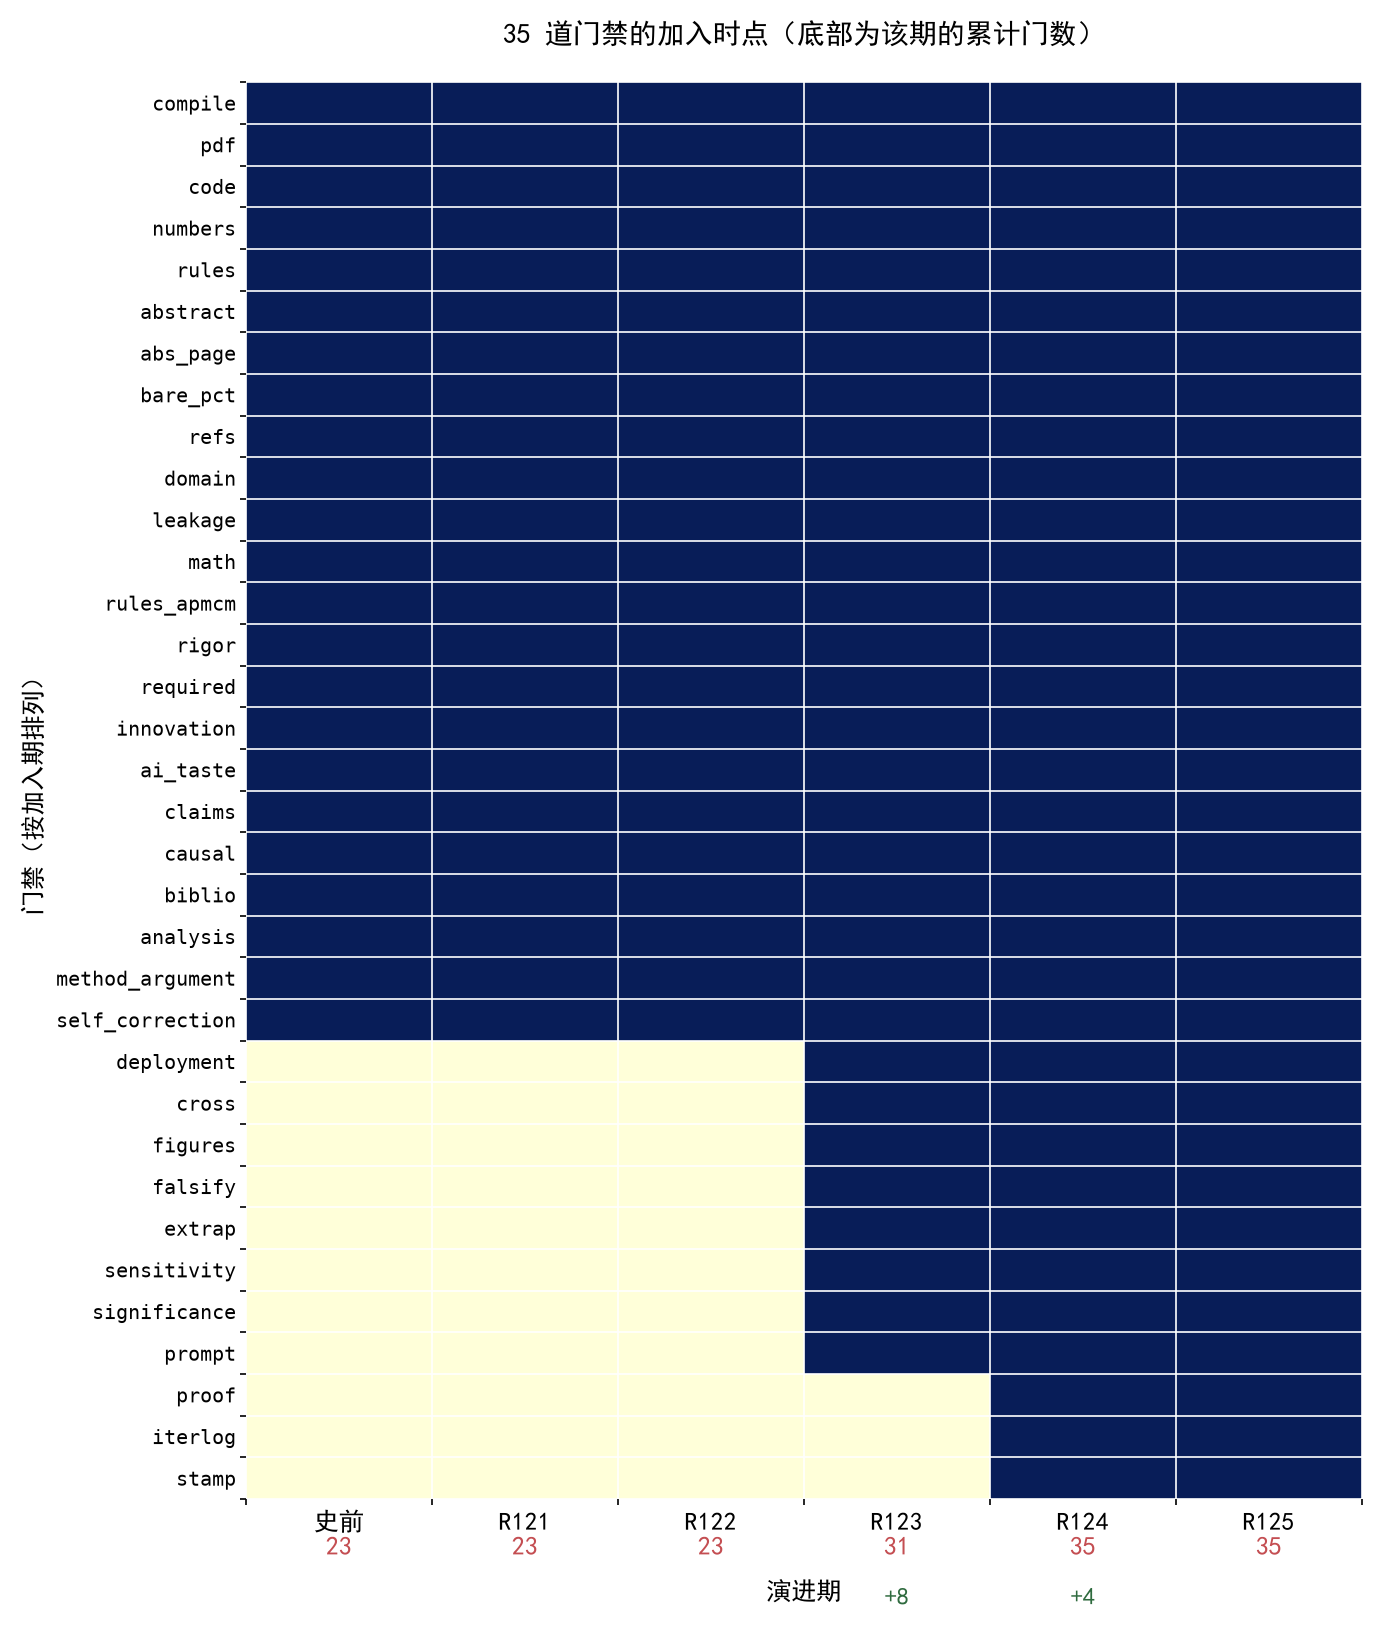
\includegraphics[width=0.70\textwidth,height=0.55\textheight,keepaspectratio]{figs/figI_heatmap.png}
\caption{35 道门禁的加入时点。每一行是一道门，颜色越深表示该期已存在；底部两行数字分别是累计门数与本期新增。\textbf{这张图说明扩容不是均匀的}：R123 一次加了 8 道、R124 加了 4 道，其余三期一道没加——每一次跳跃都对应一个具体事故，没有一次是计划性扩张。}\label{fig:gatesheat}
\end{figure}

表 \ref{tab:phases} 是本文的骨架。末列只写\emph{文件系统里真的留下了时间戳}的项；其余标「未记录」——按本文的判据，没有记录的时间不能事后追认为摘要，只能如实标空。每一期的“触发”都是一个具体事件，而非计划。前四期改的是“门做什么”，第五期改的是“门是什么”（图~\ref{fig:gategrowth}）（图~\ref{fig:gatesheat}）。

\begin{table}[tbp]\centering\small
\caption{演进分期：每期由什么触发，加了什么，代价是什么}\label{tab:phases}
\setlength{\tabcolsep}{3pt}
\begin{tabular}{p{1.1cm}p{2.9cm}p{4.0cm}p{3.4cm}p{2.2cm}}
\toprule
期 & 触发事件 & 主要改动 & 留下的问题 & 可考时间\\
\midrule
史前 & 需要算得对 & 能力层 23 命令、验证三件套、门禁初版 23 项 & 门禁靠记忆列，无比例约束 & 未记录\\
R121 & 论文 12 节而名单只有 7 板 & 板数改为解析 \code{\textbackslash section} & 只改了代码，没有核对历史 & 未记录\\
R122 & 发现 7 个角色掩盖 5 段未审正文 & 比例关系钉进自检（4/12/20/21 节） & 门禁本身仍未被检验 & 未记录\\
R123 & 用户要求“手工检查变成规则” & 题面落地门、显著性门、文献与图的下限、逐字核对规矩 & 围栏有效性仍无举证标准 & 未记录\\
R124 & 外部评审批“用可核对方程替换了证明” & \code{proof} 门、\code{iterlog} 门、图的内容检查、转义校验 & 35 项里仅 4 项有构造缺陷 & 11-12 05:14、11-12 12:40\\
R125 & 自问“35 项里几道被证明过有效” & 四层结构（内容三层 + 元层）、域无关性、L3/L4 分离、检测--诊断--修复闭环 & X 只 4/35；L4 未实现；缺远域 & 11-12 20:54（本文）\\
\bottomrule
\end{tabular}
\end{table}

\subsection{一次自欺的形状}\label{sec:selfdeception}
在展开各期细节前，先说清 R122 暴露的那种失效，因为它是全文的原型。

\textbf{症状}：门禁报“七板七角色，13 条 finding 且均已关闭”，全绿。
\textbf{事实}：论文有 12 个 \code{\textbackslash section}，5 段正文（题面重述、假设、符号说明、
自我评价、结论）\textbf{从来没有独立审核者}。
\textbf{机理}：审核名单是一个\textbf{硬编码的常量}（7），而它要覆盖的对象是一个\textbf{变量}（12 节）。
当常量小于变量时，多出来的部分\textbf{静默地不存在于检查范围内}——不是失败，是根本没被看见。

这件事给出全文的判据：\textbf{一个绿灯只在“指标的分母等于对象”时才有意义。}
后文 §\ref{sec:r123} 的“题面必须落地”、§\ref{sec:mutation} 的变异测试，
都是这条判据的不同实现。

%==================================================== 3
\section{史前：先把“算得对”这件事拿下来}

\subsection{起点不是护栏，是计算}
这套系统的第一版\textbf{没有任何门禁}。它只有一件事要做：让“算出来的数”是可信的。
当时的判断很朴素——如果模型连回归系数都算错，讨论“溯源”毫无意义。
于是先建能力层。

能力层的形态是一个统一入口加若干子命令。到本文统计时，
\code{schema.json} 登记的命令数是 \textbf{23} 个：

\begin{center}\small
\code{advise} \code{ahp} \code{clean} \code{cluster} \code{contract} \code{dim}
\code{experiment} \code{forecast} \code{fuzzy} \code{graph} \code{grey}
\code{greyrel} \code{hints} \code{merge} \code{ode} \code{plot} \code{profile}
\code{race} \code{run} \code{selftest} \code{skeleton} \code{solve} \code{video}
\end{center}

覆盖的数学结构包括：描述统计与数据剖面、回归与分类拟合、时间序列预测（含灰色预测）、
约束优化与多目标帕累托、层次分析、模糊综合评价、灰色关联、聚类、
图论四类（最短路/最小生成树/最大流/旅行商）、常微分方程、量纲分析、
以及十六类图形输出。\\[2pt]
\textbf{这个清单不是设计出来的，是长出来的。}每一类都是因为某个具体题目
逼出来的，而不是先有“建模全谱”的框架再去填。

\subsection{把“算”与“写”切开}
能力层有一条从一开始就定死、后来再没变过的规矩：
\textbf{能力层从不写散文，决策层从不算数。}

这条规矩针对一个具体失效：当同一主体既算数又写叙述时，会出现“把叙述悄悄调到
与某个它并未真正产生的数字相匹配“的情况。分开之后，正文里的每个数都必须
从一个命令的输出里取，而命令的输出与正文的措辞之间没有回旋余地。

代价是接口设计的成本——每个能力必须以可被引用、可被复核的形式输出数字
（而不是一段结论）。这个代价后来被证明是必要的：正因为输出是数字而非句子，
§\ref{sec:mutation} 的溯源检查才有对象可查。

\subsection{第一次被自己的数字打脸：例子是编的}
能力层建好之后，论文开始有数字了，紧接着出现了第一次真实事故。
这次事故值得完整记录，因为它暴露了后来所有门禁都要对付的那个盲区。

在一段说明“报告里的数字分几类”的正文里，我们写了这样一句：

\begin{quote}\small
取热沉报告的一页：它印着六位小数的拟合系数、一个\textbf{编号为 12 的表行}、
一个从输入文件抄来的\textbf{年份 2019}，以及一个\textbf{显著性水平 0.05}。
\end{quote}

事后逐字核对的结果见表 \ref{tab:fabricated}。

\begin{table}[tbp]\centering\small

\caption{四个例子的逐字核对结果}\label{tab:fabricated}
\setlength{\tabcolsep}{4pt}
\begin{tabular}{p{4.2cm}p{8.2cm}}
\toprule
正文声称 & 核对结果\\
\midrule
六位小数的系数 & \textbf{真}：\code{0.007434} 确实存在于该报告\\
“年份 2019” & \textbf{编造}：该报告 0 次命中，这篇根本没有年份列\\
“编号 12 的表行” & \textbf{错认}：\code{12} 是帕累托表第一列的\textbf{设计编号}，不是行号\\
“显著性水平 0.05” & \textbf{错认}：实际是 Breusch--Pagan 检验的\textbf{临界值}\\
\bottomrule
\end{tabular}
\end{table}
数字分类的原始洞察来自一张解剖表：把语料里每个数值 token 按“合法来源”分堆。
需要说明的是，那张表用的是\emph{旧口径}（5\,822 个 token、五类，含“表格抄录值”），
本文用的是\emph{新口径}（9\,337 个 token、四类，见第 \ref{tab:genre} 节）。
两套口径的差别本身就是一条证据：\textbf{分类器改过一次，而改动的理由是旧的第五类无法机械判定}。

\textbf{四个例子，两个是编的、两个是错认的，而当时所有检查全绿。}
原因是两个盲区叠加：
\begin{enumerate}[leftmargin=1.6em,itemsep=2pt]
\item \code{\textbackslash code\{\}} 里的字面量被分词器整体空白化，里面的数字不进判定；
\item 整数本来就不在“数字溯源”的判定范围内（只判带小数的 token）。
\end{enumerate}
两者相乘，恰好覆盖了“举例用的整数”，而举例正是最容易编造的地方。

这件事直接催生两条规矩（§\ref{sec:r123}）：\textbf{引用某个文件里的数必须到那个文件里逐字 grep 一次}；
\textbf{举假想例子必须写明 \code{for instance}，不得写成 \code{the report prints}}。

\subsection{验证三件套}
在同一时期定形的还有三个验证工具，它们后来成为每次改动的标准动作：

\begin{table}[tbp]\centering\small
\caption{验证三件套与门禁的分工}\label{tab:triad}
\setlength{\tabcolsep}{4pt}
\begin{tabular}{p{2.05cm}p{5.5cm}p{5.9cm}}
\toprule
工具 & 回答什么 & 不回答什么\\
\midrule
\code{verify.py} & 正文里每个数能否追到一次计算 & 追到的那个数是否被正确解释\\
\code{falsify.py} & 主动找反例：滑窗内有无符号相反的区间 & 反例之外另有什么\\
\code{lanes.py} & 多通道并行验证（交叉验证/自助/留出/残差/外推/扰动/对抗）投票 & 通道本身选得对不对\\
\code{gate.py} & 稿子能否交付（35 项结构性与语义性检查） & 论证是否成立\\
\bottomrule
\end{tabular}
\end{table}

\subsection{史前期的真实缺口}

\begin{figure}[tbp]\centering
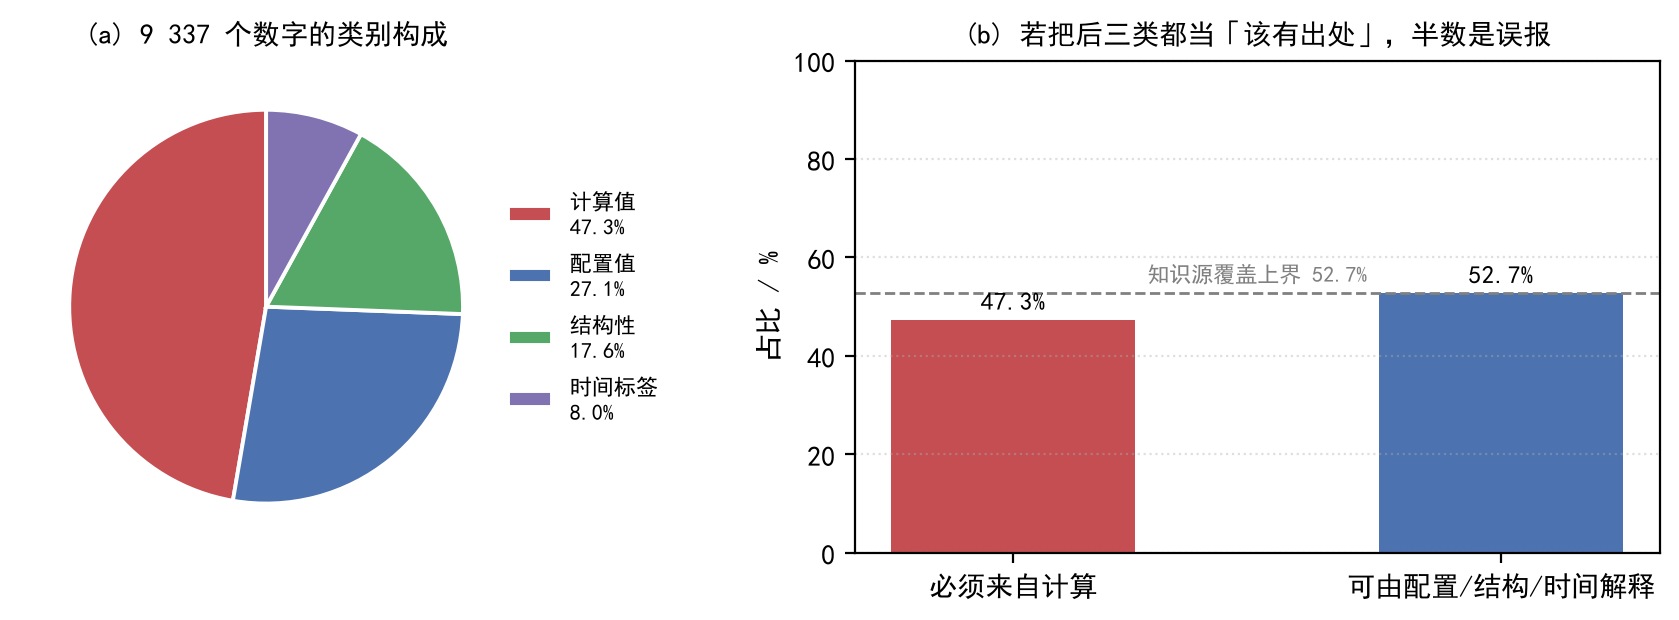
\includegraphics[width=0.92\textwidth]{figs/figC_genre.png}
\caption{9\,337 个数字的类别构成。(a) 只有 47.3\% 是计算值；(b) 若把配置、结构、时间三类也都当成「该有出处」，则近半数告警是误报。这是「需要计算谱系判据」而非「需要更强知识库」的量化依据。}\label{fig:genre}
\end{figure}

\begin{figure}[tbp]\centering
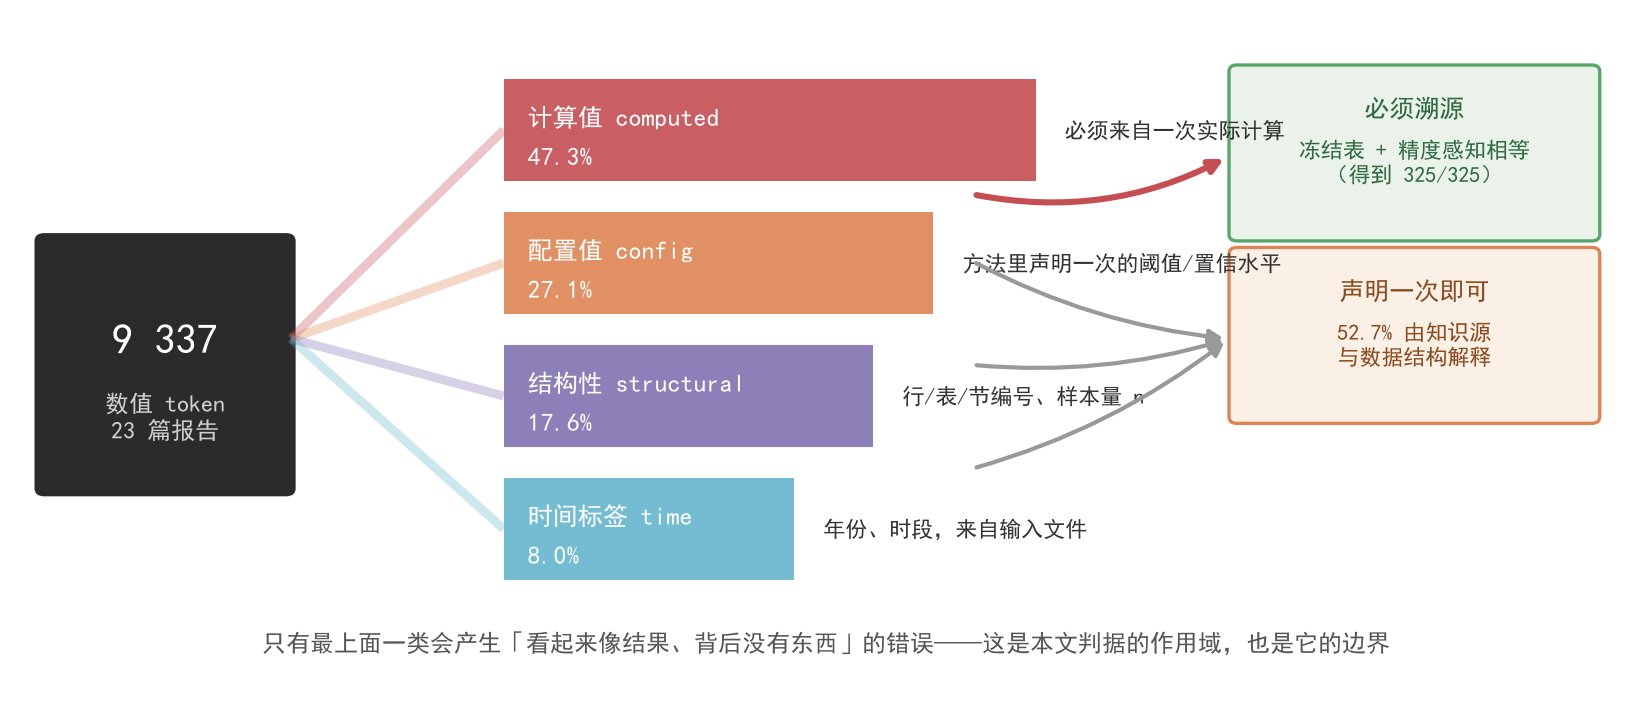
\includegraphics[width=0.98\textwidth]{figs/figG_flow.png}
\caption{9\,337 个数值 token 的流向。四类各有合法来源，但只有计算值一类会产生“看起来像结果、背后没有东西”的错误——这是判据的作用域，也是它的边界。右侧两个出口对应两种处置：计算值必须落进冻结表，其余三类声明一次即可。}\label{fig:flow}
\end{figure}

这一期结束时，能力层可用、数字可溯源、有了一版 23 项门禁（表~\ref{tab:triad}）。数字如何分类见图~\ref{fig:genre} 与图~\ref{fig:flow}——分类是这一期最重要的副产品，因为它决定了后面所有判据的作用域。但有三件事没做。
它们构成后三期的起点：

\begin{enumerate}[leftmargin=1.6em,itemsep=2pt]
\item \textbf{门禁项是凭记忆列的}，没有任何机制保证“该查的都查了”；
\item \textbf{门禁自身从未被检验}——它报绿，不等于它有检出能力；
\item \textbf{写完文件不做校验}，而写文件的通道（PowerShell heredoc）会静默改写字符。
\end{enumerate}

%==================================================== 4
\section{第一次转折（R121--R122）：从固定名单到比例约束}

\subsection{R121：板数不该是常量}
触发很简单：论文有 12 个 \code{\textbackslash section}，而红队审核名单里只有 7 个角色。
当时的做法是让审核名单可配置、列宽自适应、slug 去重，
并允许用 \code{disposition} 代替 \code{resolved} 来关闭一条 finding。
这些都是工程修缮，问题没有暴露。

\subsection{R122：七个人审了十二节}
真正的问题在下一轮被自己的自检抓出来：
\code{redteam.py} 的 \code{SPEC} 列出 7 个板块，而 \code{paper.tex} 有 12 节。
\textbf{五段正文从来没有审核者}——分别是题面重述、模型假设、符号说明、
自我评价与扩展、结论。而门禁仍然报“七板七角色，13 条 finding 且均已关闭”。

这个失效的结构值得拆开看，因为它在别处会以别的形状重复：

\begin{enumerate}[leftmargin=1.6em,itemsep=2pt]
\item \textbf{对象是变量}：$\text{板块数} = \#\{\code{\textbackslash section}\}$，随稿子变化；
\item \textbf{指标是常量}：审核名单写死 7；
\item \textbf{比较被省略}：没有任何代码去断言“名单长度 == 节数”。
\end{enumerate}

于是在 $12 > 7$ 时，多出的 5 节\textbf{不是“审核失败”，而是“不存在于检查范围”}。
门禁无法报告它，因为门禁自己也不知道有 5 节没被覆盖。

\subsection{修法与它为什么必须钉进自检}
修法是把比例关系写成断言，并且\textbf{用不同规模的样本反复验证这条断言本身}：
\code{redteam.py selftest} 用 4 节、12 节、20 节、21 节四篇最小论文，
确认“需要几个审核者”随节数严格变化，且角色不得复用。

\begin{proposition}[比例约束的必要性]\label{prop:ratio}
设论文有 $S$ 节、审核名单有 $R$ 个角色。若 $R$ 是一个与 $S$ 无关的常量，
则当 $S > R$ 时，$S - R$ 节正文无审核者，且门禁报告为全绿。
\end{proposition}

\begin{proof}
门禁只遍历名单（$R$ 个元素），不遍历节（$S$ 个元素）。
$S > R$ 时节集合中必有元素不在名单的像里，该元素不被任何检查访问，
故不产生 finding；而所有被访问的元素均通过，故整体状态为通过。
\end{proof}

命题 \ref{prop:ratio} 平凡，但它的工程含义不平凡：\textbf{任何“用一个常量去覆盖一个变量”
的检查，都会在变量变大时静默失效。}这类检查的正确实现必须让分母从对象本身导出。

\subsection{这一期的教训}
R121--R122 留下的不是一条规矩，而是一条\textbf{判据}：
看到一个绿灯，先问“它的分母是什么，分母是怎么来的”。
如果分母是手写的，绿灯不可用。

这条判据在下一期被应用到三个新地方：题面、例子、文献。

%==================================================== 5
\section{第二次转折（R123）：把手工检查变成规则}\label{sec:r123}

\subsection{触发：两句用户指令}
这一期的起点不是我们自己发现的问题，而是两条明确要求：
\begin{quote}\small
「要约束 LLM 认真地读取题目信息，不允许猜，不允许跳过！」
「凡是手工检查的，都应该变成规则。」
\end{quote}

第二条要求把一类工作从“每次靠记性”变成“每次靠程序”。下面按落地顺序记录。

\subsection{题面必须落地、逐字引用、逐问回应}
原来的状态是：\code{paper.tex} 里有 \code{\textbackslash section\{Restatement of the problem\}}
就算通过，而这一节\textbf{完全可以凭记忆写}。

实测证据：某份竞赛稿的目录里\textbf{没有任何题面原文}，
正文的“What the problem asks”是转述。转述不必然是错的，
但\textbf{无法核实它是否忠实}——读者不知道题面是不是真的这么问。

新增门 \code{chk\_prompt}（当时第 33 项）三条判据：

\begin{table}[tbp]\centering\small
\caption{\code{chk\_prompt} 的三条判据}\label{tab:prompt}
\setlength{\tabcolsep}{4pt}
\begin{tabular}{cp{6.4cm}p{6.2cm}}
\toprule
& 判据 & 抓什么\\
\midrule
A & \code{out/<dir>/题目.md}（或 \code{prompt.md}/\code{题目.txt}）存在且 $\ge 200$ 字符 & 题面没落地 →「认真读题」无从核实\\
B & 正文 Restatement 中 $\ge 40$ 字与题面\textbf{逐字连续一致}（比对前归一 \LaTeX{} 转义与空白） & Restatement 是凭空转述\\
C & 题面的编号小问（\code{(1)}/\code{1.}/\code{Problem 1}/\code{问1}）\textbf{全部}在正文被回应 & \textbf{跳过某一问}\\
\bottomrule
\end{tabular}
\end{table}

\code{--seed} 的能力边界也被实测钉住：\code{runs.json} 的 \code{problem} 字段只有
9--52 字符（\code{heat sink}、\code{forecast monthly sales from price and advertising}），（表~\ref{tab:prompt}）
那是\textbf{题名}不是原文。所以 \code{--seed} 写出的 \code{题目.md} 只有 100 来字节，
\textbf{过不了 A 条的 200 字符门槛——补原文是人的活，程序不能编。}

两份交稿在这条门上\textbf{都是红的}，这是正确结果：

\begin{center}\small
\begin{tabular}{ll}
\toprule
目录 & 判定\\
\midrule
\code{out/final} & FAIL：没有题面原文\\
\code{out/d2026c} & FAIL：题面只有 112 字符（$<200$）；正文与题面无 40 字以上逐字一致片段\\
\bottomrule
\end{tabular}
\end{center}

\subsection{例子必须逐字核对}
对应 §3.3 的事故。落成规矩是：

\begin{table}[tbp]\centering\small
\caption{例子的核对义务}\label{tab:example}
\setlength{\tabcolsep}{4pt}
\begin{tabular}{p{4.4cm}p{8cm}}
\toprule
要写 & 必须做\\
\midrule
引用某篇报告里的数/标识符 & 到\textbf{那个文件}里逐字 grep 一次，确认行号\\
举一个假想的例子 & 正文写明 \code{for instance} / \code{say}，不要写 \code{the report prints}\\
用 \code{\textbackslash code\{\}} 包 & 它逃过 \code{numbers} 门，所以\textbf{更要核对}\\
\bottomrule
\end{tabular}
\end{table}

工具 \code{example\_audit.py} 列出所有 \code{\textbackslash code\{\}} 含数字的项，（表~\ref{tab:example}）
报每个字面量在哪些工件里找到。但工具的能力边界同样被写清楚：
\textbf{“找到 $\ne$ 对”}——\code{12} 在 36 个文件里都有，\code{0.05} 在 27 个里都有。
工具能证明“这个字面量存在于语料”，\textbf{不能证明它出现在正文声称的那一篇里}。
最后一步只能靠人。

\subsection{先查文献再动手}
这一条是本期最刺眼的教训，因为它否证了前 12 轮里我们自己的四个“创新”。

规则：\textbf{凡要引入一个方法论，先搜它的学术名称，再动手。}
自己推理一遍的代价不是“慢”，是\textbf{漏掉已知的反例}。

\begin{table}[tbp]\centering\small
\caption{我们“自己推出”的四件事与文献的对照}\label{tab:literature}
\setlength{\tabcolsep}{3pt}
\begin{tabular}{p{5.2cm}p{7.4cm}}
\toprule
我们自己推出的 & 文献里已有的，且更严格\\
\midrule
“改坏检查看测试是否报错” & \textbf{mutation testing}（Jia \& Harman, IEEE TSE 2011）\\
“12 个样本里 11 个通过不能当点估计” & \textbf{mutation score confidence}（Holling et al., ICSTW 2016）：分数是估计量，有置信区间\\
“多个独立审核者” & \textbf{multiversion programming}（Knight \& Leveson 1986）：\textbf{独立实现并不独立}，共用同一底座模型的多个 agent 更不独立\\
“结论在参数域上恒成立” & \textbf{metamorphic testing}（Chen et al.）与 \textbf{global sensitivity indices}（Sobol 2001）\\
\bottomrule
\end{tabular}
\end{table}

最刺眼的是第三行：我们把“12 板独立审核”当优点写进了论文，（表~\ref{tab:literature}）
而 Knight--Leveson 1986 早就否证了那个前提。这不是“表述不严谨”，
是\textbf{一个被引用了四十年的否证被我们忽略了}。
同类的方法还有蜕变测试~\cite{ref4}与全局敏感性指数~\cite{ref5}，前者用于生成下一批测试用例，后者用于判断结论在参数域上是否恒成立。


\subsection{交付标准的四项门槛}
用户要求“不是只有这篇论文，而是用这个插件必须遵循如此的规则”。
于是四条写进 \code{gate.run\_all}，对每一份 \code{deliverable} 生效：

\begin{table}[tbp]\centering\small
\caption{交付标准四项门槛及其依据}\label{tab:delivery}
\setlength{\tabcolsep}{3pt}
\begin{tabular}{lp{3.2cm}p{5.2cm}p{2.6cm}}
\toprule
门 & 门槛 & 为什么 & 覆盖方式\\
\midrule
\code{refs} & $\ge 10$ 条文献且每条有 \code{\textbackslash cite} & 评委据此判断作者读没读过这个领域 & \code{standard.json} 的 \code{min\_bib}\\
\code{figures} & $\ge 6$ 张图 & 只查质量不查数量，“4 张图 + 9 张表”会拿满分 & \code{min\_figs}\\
\code{sensitivity} & 实质性三件：表述 + 参数范围 + 扰动后判断 & 敏感性分析是分水岭；只查关键词会被堆词通过 & 缺哪件点名缺哪件\\
\code{significance} & 区间/误差数值，且\textbf{不能是定义域}（如 $[0,1]$） & 对应 NeurIPS~\cite{ref9} 清单第 7 项：只给点估计等于不知道自己多不确定 & 平凡区间在代码里排除\\
\bottomrule
\end{tabular}
\end{table}

门槛值本身是设计选择不是定理（优秀论文的文献量/图数只有经验区间），（表~\ref{tab:delivery}）
所以做了三件事：写成模块常量可被 \code{standard.json} 覆盖；
结论行打印“实际值 / 门槛”；只对 \code{\_is\_deliverable} 为真的目录生效。

\subsection{一个不写声明就静默豁免的坑}

R124 之前门禁是 33 项，扩容到 35 项的过程见附录的完整清单
（第 \ref{sec:deficit} 节后的两张表）。\textbf{此处不复印旧版截图}：
旧清单的价值只在于“记录每一项为什么存在”，而那份理由已经并进正文各节的触发事件里。

这是本期最危险的一处，因为它让\textbf{所有交付标准同时失效}。

实测：一份 17 页手工竞赛稿的 \code{declaration.json} 只写了 \code{no\_dataset}，
\textbf{没写 \code{deliverable}}。结果文献下限、图数下限、敏感性门、红队分板
\textbf{四道全不生效}，门禁报“4 张图 8.0/10”，看起来比交稿还漂亮。

补上 \code{"deliverable": true} 之后，它立刻暴露 5 个真缺陷：

\begin{center}\small
\begin{tabular}{llp{8.4cm}}
\toprule
门 & 判定 & 内容\\
\midrule
\code{numbers} & FAIL & 70/72，且冻结表没写 \code{generated\_from}（交稿要求能追到生成它的脚本）\\
\code{refs} & FAIL & 全文 0 条 \code{\textbackslash cite}\\
\code{redteam} & FAIL & 没有 \code{redteam.json}：论文 12 个板块都没有审核记录\\
\code{figures} & FAIL & 只有 4 张图，低于交付下限 6 张\\
\code{sensitivity} & OK & 有扰动范围（3 处）且有扰动后的判断\\
\bottomrule
\end{tabular}
\end{center}

其中 \code{generated\_from} 与 \code{redteam} 两条，\textbf{在补声明之前完全看不见}。

规矩由此确立：\textbf{新建任何准备拿出去的目录，第一步写 \code{declaration.json} 且带 \code{"deliverable": true}}；
不写就是“草稿”，所有交付标准静默豁免。

%==================================================== 6
\section{第三次转折（R124）：图从来没有被打开看过}\label{sec:r124}

\subsection{触发：一句外部评审意见}
外部评审对工具论文的批评只有一句，但准确：
\textbf{“把证明换成了一段可核对的方程。”}
核实后确认属实，于是暴露一个结构性缺口：35 道门里，
\textbf{没有任何一道问“关键推导是否被写成命题并给出证明”。}

顺着这个逻辑继续查，又发现第二处同类缺口。

\subsection{图的技术分不是内容分}
\code{figcheck} 只看技术规格：DPI、尺寸、背景色、长宽比、是否矢量。
\textbf{它不打开任何一张图看里面画了什么。}
当它报“均分 8.0/10（24 张）”时，给人的印象是“图都很好”——
而那是\textbf{技术分，不是内容分}。

实测踩到两类内容缺陷：
\begin{enumerate}[leftmargin=1.6em,itemsep=2pt]
\item \textbf{图内标题与 caption 说同一句话}：matplotlib 的 \code{ax.set\_title(...)}
  与 \LaTeX{} 的 \code{\textbackslash caption\{...\}} 意思重叠，读者在图上方和下方各读一遍。
  A/B 那四张图就是这样，被外部评审点出来。
\item \textbf{孤立图}：定义了 \code{\textbackslash label\{fig:x\}} 但正文一次没有 \code{\textbackslash ref\{fig:x\}}。
\end{enumerate}

新增 \code{tools/fig\_visual.py} 做两道可机械判的检查，相似度按
“去停用词后的词重叠 / 较短句词数”计算（不是编辑距离），阈值 0.75 判“几乎逐字重复”、
0.45 判“意思重叠”。

\subsection{这个检测器自己错了两次}
这是本文反复出现的模式：\textbf{新写的检查器本身需要先被检查。}

\begin{table}[tbp]\centering\small
\caption{\code{fig\_visual} 的两次自身缺陷}\label{tab:figbug}
\setlength{\tabcolsep}{4pt}
\begin{tabular}{p{5.2cm}p{4.2cm}p{4.2cm}}
\toprule
症状 & 原因 & 修法\\
\midrule
24 张图的相似度全部为 0.00 & 按\textbf{脚本文件名}匹配图与脚本，而脚本名不含图名 & 改为映射 \code{savefig} 的输出路径\\
随后出现 4 个误报 & “所有标题 $\times$ 所有 caption”两两比较 & 只在\textbf{所属脚本}的标题范围内比较\\
\bottomrule
\end{tabular}
\end{table}

\subsection{机械检查做不到的部分}
工具会打印“逐张人工核对清单”，但清单本身不是执行。至少五项必须人看，见表~\ref{tab:figbug}
坐标轴标签缩到论文宽度后是否可读；图里是否真有数据（不是空白或只有框架）；
图与正文是否一致（正文说上升，图里不能是平的）；边距是否裁掉标签或图例；
黑白打印时颜色是否还能区分。

\textbf{这里必须记一条诚实的欠账}：这条规矩写成之后，
“24 张图逐张打开看”这个动作\textbf{并未执行}（见 §\ref{sec:deficit} 的清单第 3 项）。
规矩与执行之间的差距，本文不掩饰。

\subsection{写文件会被静默改写}
本期最后一个缺口与内容无关，与\textbf{通道}有关。

本项目的写文件操作有一半是经 PowerShell 的 heredoc（\code{@"..."@}）传给 python 的。
而 PowerShell \textbf{用反引号做转义}，于是下列字符被静默改写：

\begin{table}[tbp]\centering\small
\caption{PowerShell heredoc 的静默转义（实测）}\label{tab:escape}
\setlength{\tabcolsep}{4pt}
\begin{tabular}{lll}
\toprule
写了 & 变成 & 后果\\
\midrule
\code{`a} & \textbf{BEL}（\code{\textbackslash x07}） & 看不见，但 \code{`aidc2026} 变成 \code{<BEL>idc2026}\\
\code{`t} & \textbf{TAB}（\code{\textbackslash x09}） & 在 Markdown 表格里破坏对齐\\
\code{`b} & \textbf{BS}（\code{\textbackslash x08}） & \code{`baidu} 变成 \code{<BS>aidu}\\
\code{`f} & \textbf{FF}（\code{\textbackslash x0c}） & \code{`falsify} 变成 \code{<FF>alsify}\\
\code{`n} & \textbf{LF} & 字符串里凭空多一个换行\\
\bottomrule
\end{tabular}
\end{table}

实测踩到 6 次，其中 3 处污染\textbf{一直留到了 v8 和 README 里}，（表~\ref{tab:escape}）
是由写后校验工具抓出来的——\code{analysis}、\code{falsify}、\code{ai\_taste}
三个词的开头各被吃掉。

由此确立两条规矩，一条靠记性、一条不靠：
\begin{enumerate}[leftmargin=1.6em,itemsep=2pt]
\item 含反斜杠、反引号、引号的内容，用直接写文件的方式，\textbf{不经过 shell}（第一道防线，靠记性）；
\item 写完跑 \code{check\_write.py}（兜底，不靠记性）。
\end{enumerate}

\code{check\_write.py} 抓六类：控制字符（BEL/NUL/BS/FF/ESC）、
\code{.md}/\code{.json}/\code{.txt} 里的 TAB、零宽字符（\code{\textbackslash u200b} 等）、
UTF-16 BOM（\code{out/} 下 48 个 \code{.txt} 就是这样，因为 PowerShell 的 \code{>} 默认写 UTF-16）、
CR/LF 混用、BOM 出现在文件内部。
它的自校用 4 个\textbf{构造样本}（1 干净 + TAB/BEL/零宽各 1），而不是读当前文件——
这一点很重要，理由见 §\ref{sec:mutation}。

%==================================================== 7
\section{第四次转折（R124 末--R125）：从“门”到“层”}\label{sec:layers}

前三次转折改的都是“门做什么”，这一次改的是“门是什么”。
转折的触发不是外部评审，而是一个自问：\textbf{35 道门里，究竟几道被证明过有效？}

\subsection{触发：一个把自己判负的实验}

前四期一直在加门，从 23 项加到 35 项。R124 末第一次停下来数：
35 项里，有多少项同时具备\emph{构造出的缺陷样本}与\emph{变异测试敏感}这两件事？

做法是把两个已有仪表的覆盖面对起来：
\code{fence\_acceptance.py} 的 12 个构造样本，\code{fence\_mutation.py} 的 4 个变异，
各自打到哪几道门上。

\begin{table}[tbp]\centering\small
\caption{35 项门禁的验证覆盖（R124 末实测）。X 类有构造缺陷且经变异测试；Y 类只有判据实现。}\label{tab:xy}
\setlength{\tabcolsep}{3pt}
\begin{tabular}{p{1.5cm}p{2.6cm}p{7.4cm}p{2.2cm}}
\toprule
类 & 门 & 凭什么算这一类 & 数量\\
\midrule
X & \code{numbers} \code{figures} \code{redteam} \code{stamp} &
\code{fence\_acceptance} 的 S1--S12 分别打到：S1/S2（舍入与地板）打 \code{numbers}，
S6（旧图）打 \code{figures}，S8（工件过期）打 \code{stamp}，
S9--S12（编造 evidence、未处理当关闭、板数不符、拿错基准）打 \code{redteam}；
且四道门各有变异器 & \textbf{4}\\
Y & 其余 31 项 & 有判据代码，但没有任何构造缺陷证明它抓得住 & \textbf{31}\\
\bottomrule
\end{tabular}
\end{table}

结论是\textbf{覆盖率 4/35 = 11.4\%}。这个结果没有粉饰的余地，见表~\ref{tab:xy}
按本文 §\ref{sec:mutation} 自己立的规矩，\emph{没有构造缺陷的门不算被证明过}，
所以“35 项全绿”这句话，只在 4 项上成立。

\textbf{这一节的意义不在于承认覆盖率低，而在于：一个只会加门的系统，会系统性地高估自己。}
每加一道门的成本是十分钟，构造一个能骗过它的样本的成本是三十到六十分钟。
成本不对称，所以门的增长速度必然快于证据的增长速度——
\textbf{这不是懒惰，是结构。}

\subsection{突破一：把“计数”换成“分层”}
这套分工不是新发明：契约式设计\cite{ref19}把前置/后置条件写进代码，运行时验证\cite{ref20}在执行中检查断言，Hoare 逻辑\cite{ref21}给出证明义务。本文的差别只在\emph{对象}——它们检查程序，本文检查一份报告里的数字与推导。


35 是一个\emph{计数}。计数的问题是：它无法回答“够不够”，只能回答“有多少”。
审稿人问“为什么不是 50 道”，答不上来；问“为什么不是 20 道”，也答不上来。

R125 的第一个动作是把 35 项按\emph{它们检查的对象}重新归类，得到三层。\textbf{这里的“层”与第 \ref{tab:layers} 节的“三个组件”不是同一件事}：那里说的是\emph{谁干活}（作者、能力层、验证层、门禁），这里说的是\emph{检查什么}（一个值、一条推理、一次迭代）。两套划分互相正交——同一个门可以检查三个对象中的任何一个。

\begin{table}[tbp]\centering\small
\caption{四层结构与它们各自的对象。前三层是内容层，第四层是元层。}\label{tab:fourlayer}
\setlength{\tabcolsep}{3pt}
\begin{tabular}{p{0.9cm}p{1.9cm}p{2.3cm}p{3.6cm}p{4.1cm}}
\toprule
层 & 对象 & 判据 & 失败的表现 & 对应门（代表）\\
\midrule
L1 & 一个数 & 在冻结表里吗 & 数字是编的 & \code{numbers} \code{stamp}\\
L2 & 一条推理 & 有非空证明吗 & 有等式无证明 & \code{proof}\\
L3 & 一次迭代 & 有“不信判据”吗 & 事后复盘代替当下怀疑 & \code{iterlog}\\
\midrule
L4 & 一段轨道 & 连续同错/编辑距离/上下文占比 & 原地打转 & \emph{未实现}\\
\bottomrule
\end{tabular}
\end{table}

这个归类的关键不在“三层”“四层”这两个数，而在三条性质，见表~\ref{tab:fourlayer}

\textbf{(a) 三种对象不同，所以判据互不覆盖。} 值由计算产生，推理由推理产生，
过程由\emph{判断}产生（什么时候该停、什么时候该改）。可以值全对而推导错，
可以推导对而过程掩盖。

\textbf{(b) 层数有上界，且上界有理由。} 内容层到三层为止，因为第四层的候选
全部落在“不可机械判”里：假设是否合理（要领域知识）、结论是否被证据支持
（有不可能性结果~\cite{ref16}）、数据是否真实（只能查内部一致）、审稿人是否独立（只能查有没有读别的报告）。
\textbf{“到此为止”不是没做，是能做到这里为止，而且知道为什么。}

\textbf{(c) 第四层不是“更上一层的内容”，是另一个坐标轴。}
L1--L3 问的是“这份产出对不对”，L4 问的是“继续做下去有没有意义”。
对象从\emph{静态产出}变成\emph{运行轨迹}，所以它与前三层的独立性是\emph{类型独立}，
不需要构造样本证明；需要做的是让它的信号可观测。

\subsection{突破二：从“领域工具”到“作用在输出层”}

第二个发现来自一次代码统计：扫 \code{gate.py} 的 32 个 \code{chk\_} 函数体，
看有没有数学建模特定的关键词（MILP、regression、题型、聚类、灵敏度等）。

结果是\textbf{28 道不含这类关键词，占 80\%}。它们依赖的不是“数学建模”，
而是“一篇带数字、图表、推导、过程的文档”。

于是主张从\emph{枚举性}换成\emph{结构性}：

\begin{table}[tbp]\centering\small
\caption{两种“通用”的区别}\label{tab:general}
\setlength{\tabcolsep}{4pt}
\begin{tabular}{p{1.8cm}p{4.4cm}p{5.0cm}p{3.4cm}}
\toprule
& 主张 & 怎么被反驳 & 强度\\
\midrule
枚举性 & 我在 $N$ 个域验证过 & 再加一个域 & 随样本数线性增长，永远可以被拖住\\
结构性 & 我的判据不引用任何域概念 & 指出哪个判据依赖域 & 一次到位\\
\bottomrule
\end{tabular}
\end{table}

这个换法的代价是诚实的：主张“通用”就必须在\emph{至少一个“足够远”的域}验证，（表~\ref{tab:general}）
否则它只是分析。远的标准不是“多”，是\emph{差异最大}——
数学建模没有外部规范、过程可见性中等；医学有 CONSORT 25 项、有预注册。
若门禁在最不像的地方仍然成立，才说明它真的不依赖领域。

（这条尚未执行。它替换了早先“加第二语料”这个含糊的说法，但本身仍是待办。）

\subsection{突破三：用自己当失败样本}

长上下文下中间信息被忽略是已有实证的现象~\cite{ref15}。

前四期的“自欺”案例都来自过去（R122 的七板十二节、R123 的编造例子）。
R125 期间发生了一件更直接的事：\textbf{这一轮本身成了 L3 高、L4 低的实例。}

L3 是高的：这一轮写了交接文档、变更日志、六轮迭代表，记录完整。
L4 是低的：同一个转义坑踩了 6 次，页数调了 4 次，检测器自己被查出错了 7 次。

关键不在“犯了错”，而在记录的形态：\emph{记录里写的正是“我又踩了一次”}。
这说明 L3 与 L4 确实是两件事——
\textbf{一个把过程记得很清楚的系统，可以同时在同一个坑里反复跌倒。}

这一条对论文的价值在于它是\emph{真实的、非构造的}样本。
前四期的每一个例子都可以被质疑“是不是为了写论文而挑的”，这一条不能：
它发生在观测者身上，而观测者当时并没有在收集样本。

\subsection{突破四：把“检测”扩成闭环}
把一次对照当实验是有代价的——软件工程实证方法学要求样本量、随机化与效应量\cite{ref24}，而本文只有 $n=1$，所以第 \ref{sec:deficit} 节把它列进缺陷清单。


R124 的 \code{proof} 门有一个完整的前因后果，本文把它当作范式：

\begin{enumerate}[leftmargin=1.8em,itemsep=2pt]
\item \textbf{检测}：A/B 对照中，带护栏的一臂在“推导”维上输 2 分（27 对 29）。需要说明的是，两臂共用同一底座模型，按多版本编程的经典结果\cite{ref3}，它们并不独立——各维得分见图~\ref{fig:radar}，五通道重合的实测见图~\ref{fig:overlap}。
\item \textbf{诊断}：外部评审指出原因——“用可检查的方程替换了证明”。
\item \textbf{修复}：加 \code{proof} 门；此后本文自己写出第一个命题与 459 字符证明。
\item \textbf{复发检查}：门现在报 OK：1 个命题、1 个证明、最短 459 字符。同一套判据在该链路的另一篇产出上给出 \textbf{325/325}（分母 325），而在无护栏一臂上是 0/200——两组数用同一条命令算的，口径相同。
\end{enumerate}

值得强调的是\textbf{时序}：A/B 数据的时间戳是 05:14:27，\code{proof} 门是 12:40:39，
相差 7.4 小时。所以“加上门之后 A 臂这一维会更高”是\emph{推断}，不是实测——
重跑 A/B 尚未做。这一条的诚实性比它的结论更重要。

不过闭环本身是可以主张的：\textbf{这套机制能够发现自己的缺陷，并且修得动。}
四次转折里，前三次由用户指令触发（R121 的 12 节 vs 7 板、R123 的两句指令、R124 的外部评审），
这一次是\emph{系统自己数出来的}。这是从“被人指出”到“自己发现”的转变。

\subsection{这一期留下的三个问题}

\begin{enumerate}[leftmargin=1.8em,itemsep=3pt]
\item \textbf{X 只有 4/35。} 补样本是 40 分钟一件事，但一直没做。
      `proof` 与 `iterlog` 两道门本身是 R124 加的，至今没有自己的构造样本——
      这正是“用加门代替补证据”的同一个病。
\item \textbf{L4 一行代码没有。} 四层结构里，第四层只有判据和信号设计，
      没有任何实现。所以“过程不发散”目前是一个\emph{主张}，不是一个\emph{工具}。
\item \textbf{“通用”缺一个远域。} 80\% 的门不引用领域概念，这是分析；
      但没有在第二个域跑过，所以不能说“实证通用”。
\end{enumerate}

这三个问题都不是“再写一节”能解决的。它们是能否从“工具报告”升级为
“可投稿的系统性回顾”的分界线。

%==================================================== 8
%==================================================== 8
\section{方法论核心：怎么证明一道门真的有效}\label{sec:mutation}

变异分数本身是估计量，带置信区间~\cite{ref2}。

变异测试作为一种评估测试集有效性的方法，其系统性综述见~\cite{ref1}。

\subsection{先说不能被接受的东西}
本项目最贵的一条教训是一句否定：\textbf{报告“拦住了 $N/M$”不构成任何证据。}

理由是三处可以被作者自己操控：
\begin{enumerate}[leftmargin=1.6em,itemsep=2pt]
\item \textbf{样本是自己选的}——可以只挑那些门显然能拦的；
\item \textbf{期望是自己定的}——可以把“应当放行”设成“应当拦住”；
\item \textbf{判定是自己写的}——可以把门的逻辑抄进样本，让样本永远报“拦住”。
\end{enumerate}

前两条在一个作者、一个语料的前提下\textbf{无法根除}。第三条\textbf{必须根除}，
因为它是纯技术问题。

\subsection{一条可执行的判据}
一个“测试”要成立，必须同时满足两条，\textbf{缺一条就是假测试}：

\begin{definition}[有效测试]\label{def:test}
称一个测试对某道门有效，当且仅当：
\begin{enumerate}[leftmargin=1.4em,itemsep=1pt]
\item 它使用\textbf{构造出来的缺陷}（不能读已被修好的当前状态）；
\item 它\textbf{调用真实的门}（不能把门的逻辑复制进样本）。
\end{enumerate}
\end{definition}

第 2 条是关键的实现约束。复制逻辑的样本有一个隐蔽特征：
\textbf{把真门改坏，样本照样报“拦住”}。于是可执行的检验就出现了：
\textbf{改坏真门，看样本是否变成“漏检”}。

\subsection{变异测试的实现}
\code{tools/fence\_mutation.py} 把每道围栏改成“永远通过”，然后重跑对应样本：

\begin{center}\small
\begin{tabular}{lll}
\toprule
围栏 & 变异方式 & 样本应有反应\\
\midrule
\code{freeze.\_match\_written} & 改成恒真 & 从“拦住”变成“漏检”\\
\code{i11}（架构不变式） & 改成恒真 & 同上\\
\code{i12}（图旧于数据） & 改成恒真 & 同上\\
\code{numbers} & 改成恒真 & 同上\\
\bottomrule
\end{tabular}
\end{center}

\textbf{当前实测结果：假测试 0/4}，即四道门都被证明是敏感的。

\subsection{变异器自己也会错}

构造缺陷基准的做法是：把一个已知缺陷植入一篇已完成的论文，看门禁能否抓回。
这是第 \ref{sec:mutation} 节那套判据的第一次运行，结果记在该节的表里，
\textbf{不以截图形式复现}——截图的数字与本文的现行口径未必一致，而读者无法核对。

这一点必须记下来，因为它差点让我们误判。

\code{i11} 的签名带参数（\code{i11(spec=...)}）。变异写成 \code{lambda: ...} 会抛 \code{TypeError}，
而这个异常被\textbf{误读成“没变化”}——于是那道门看起来“不敏感”，实际是变异器坏了。
改成 \code{lambda *a, **k: ...} 之后 4/4 全部敏感。

这件事的形状与 R122 完全一样：\textbf{一个看起来像结论的输出，实际是工具坏了。}

\subsection{第 123 轮两次真实的自欺}

三机制依次移除的消融结果记在第 \ref{sec:deficit} 节后的表里。
那里的数字是\emph{实测输出}而不是评分，因此可以区分“机制有效”与“机制看起来有效”。
\textbf{同样不复印截图}：消融的结论在表里已经完整，截图的像素不提供额外证据。

变异测试就是在这一轮抓出两处自欺的：

\begin{table}[tbp]\centering\small
\caption{两次被变异测试抓出的假测试}\label{tab:faketest}
\setlength{\tabcolsep}{4pt}
\begin{tabular}{p{3.4cm}p{4.2cm}p{6cm}}
\toprule
自欺 & 症状 & 变异测试怎么抓\\
\midrule
复制围栏逻辑 & 把真围栏改坏，样本照样报“拦住” & 改坏 \code{freeze.\_match\_written} $\to$ 样本不变 $\to$ 假测试\\
只读当前状态 & 围栏改成“永远成立”，样本照样报“拦住” & 改坏 \code{i11}/\code{i12} $\to$ 样本不变 $\to$ 假测试\\
\bottomrule
\end{tabular}
\end{table}

\subsection{变异测试仍然证明不了的事}
一份只说“变异测试通过”的报告同样在偷懒。它\textbf{不能}证明，见表~\ref{tab:faketest}

\begin{enumerate}[leftmargin=1.6em,itemsep=2pt]
\item \textbf{未知缺陷的检出率}——样本全是已知的坑，变异测试只测“对已知坑是否敏感”；
\item \textbf{期望本身是对的}——例如“合法舍入该放行”也只是我们的判断，
  变异测试只能证明“改了门会让这个判断变化”，不能证明判断正确；
\item \textbf{门的判据是否正确实现了意图}——需要另一层人工核对。
\end{enumerate}

\subsection{禁止的写法清单}
由此产生一份\textbf{禁止表述}清单，写进项目规矩：

\begin{center}\small
\begin{tabular}{ll}
\toprule
禁止 & 改成\\
\midrule
“我检查过了，没问题” & 检查了哪几项、分母多少、哪项豁免\\
“gate 全绿，所以是对的” & 哪几项绿、分母是多少、哪几项判为不适用\\
“36/36 可溯源” & “199/199，按全 token 口径；门禁只判小数 43/43”\\
“拦住 11/12” & 附构造样本、该门报错输出、以及变异测试结果\\
\bottomrule
\end{tabular}
\end{center}

最后一条的依据：\textbf{不说明分母口径的比率是废话}。
同一份稿子的溯源率在全 token 口径下是 \code{199/199}，
在只判小数的口径下是 \code{43/43}——两个数字都对，但单独引用任何一个都会误导。

%==================================================== 8
\section{诚实缺陷清单}\label{sec:deficit}

\subsection{门禁自身的覆盖率}
第 124 轮结束时的自评是：

\begin{quote}\small
35 道门里，只有 \textbf{4 道}同时具备“构造缺陷 + 变异覆盖”
（\code{numbers}、\code{figures}、\code{redteam}、\code{stamp}）。
其余 \textbf{31 道}是判据实现，\textbf{没有独立样本}。
\end{quote}

这句话的含义要说清：那 31 道门\textbf{现在报绿，只说明当前稿子没触发它们}，
不说明它们有检出能力。它们是“有道理的检查”，不是“被检验过的测试”。

\subsection{尚未做的七件事}

\begin{figure}[tbp]\centering
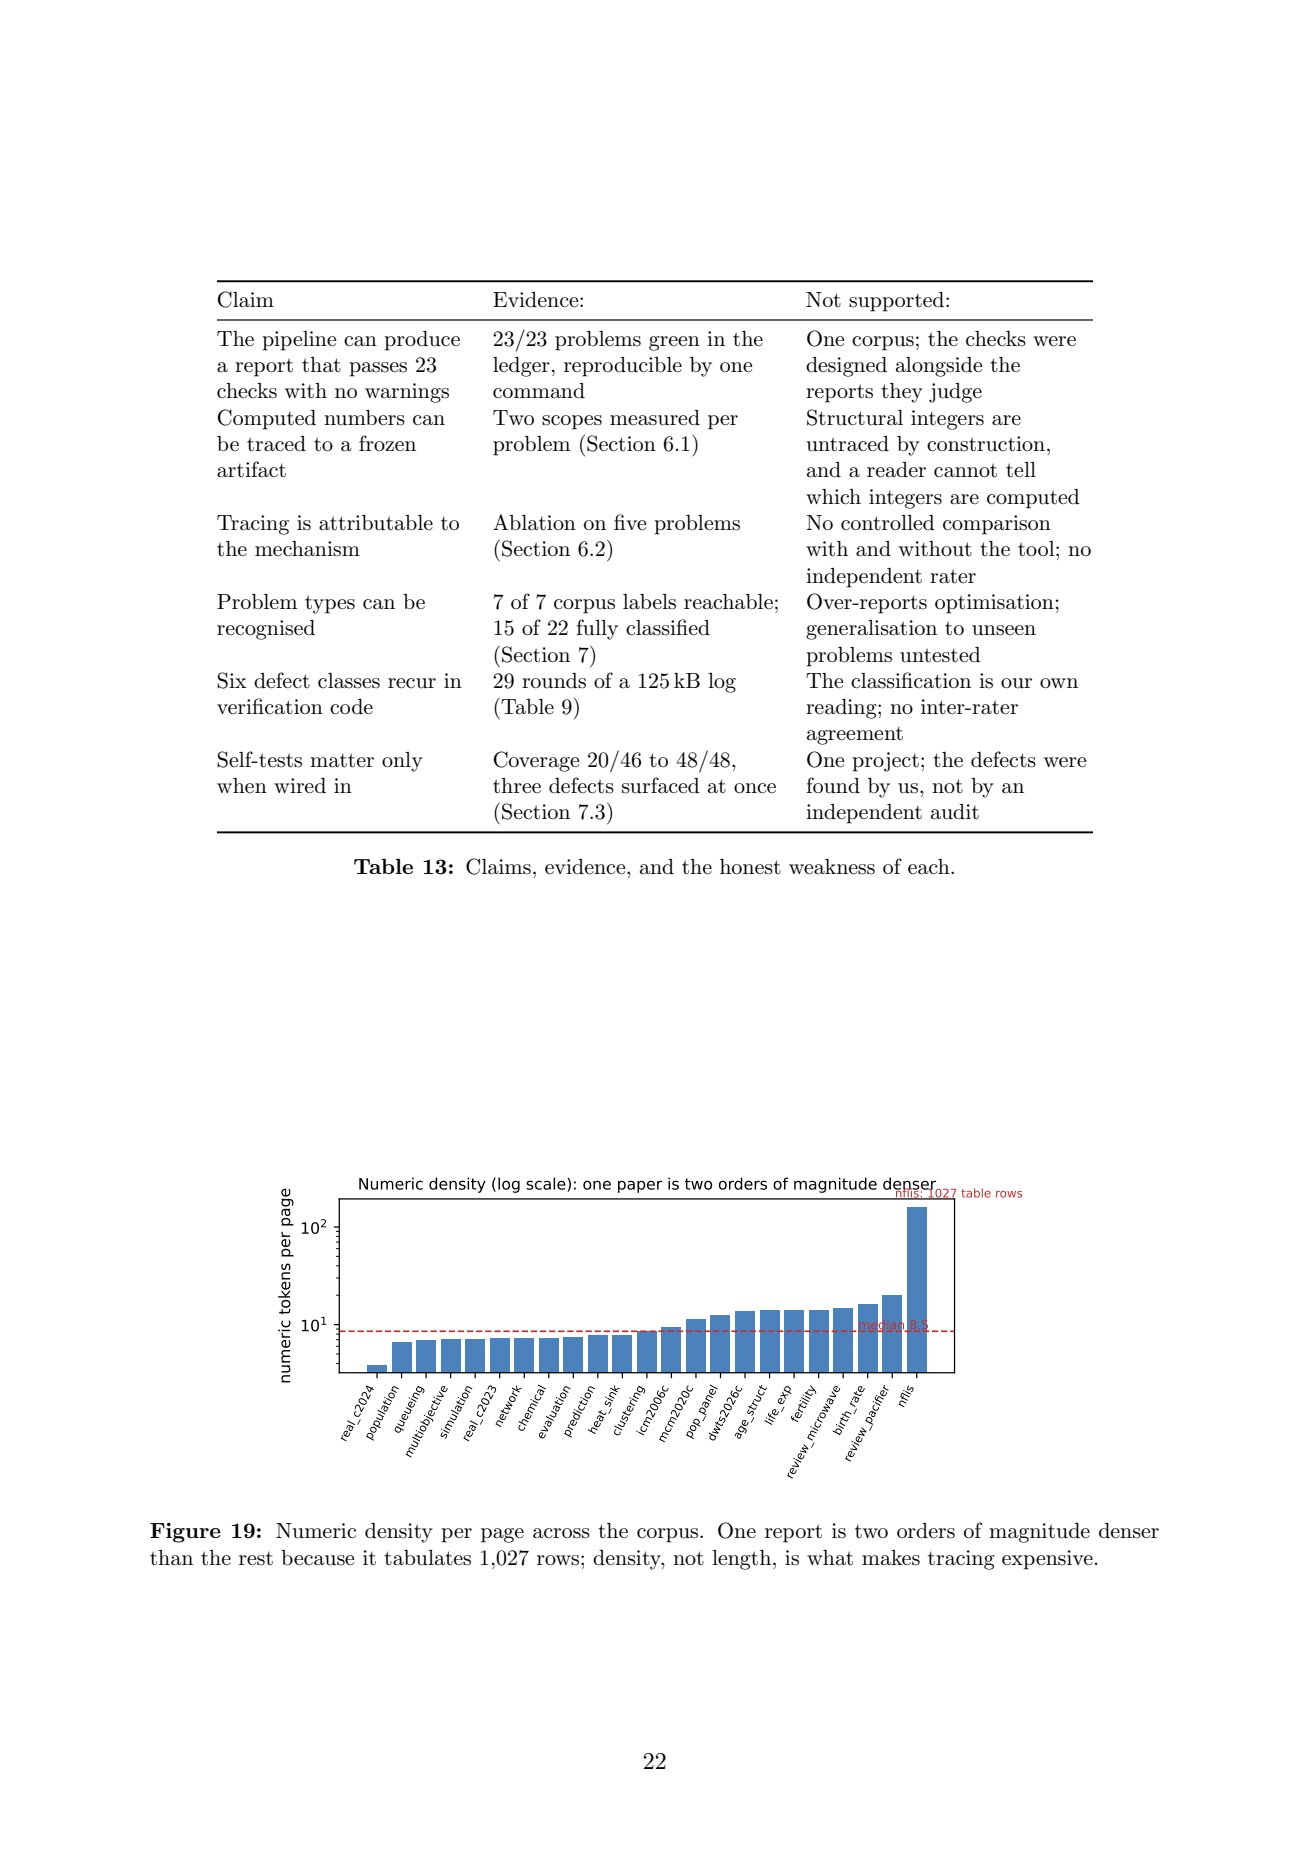
\includegraphics[width=0.60\textwidth,height=0.42\textheight,keepaspectratio]{figs/ev_not_supported.png}
\caption{早期版本中就已经存在的自我否证页（插件论文第 22 页，截图）：明确列出\emph{不被证据支持}的断言。它的存在说明「记录没做到的事」不是本文新增的姿态，而是这条链路一贯的要求。}\label{fig:notsupported}
\end{figure}

按性价比排序（表 \ref{tab:todo}）。这张表的来源是项目的交接文档，（图~\ref{fig:notsupported}）
不是事后回忆——每一条都对应一个具体判断。

\begin{table}[tbp]\centering\small
\caption{已识别但未执行的七项工作（按性价比排序）}\label{tab:todo}
\setlength{\tabcolsep}{4pt}
\begin{tabular}{cp{6.2cm}p{5.4cm}p{1.9cm}}
\toprule
\# & 做什么 & 为什么必须做 & 成本\\
\midrule
1 & 加 baseline 对比（\code{nbval} / \code{papermill} / \code{pytest --doctest-modules}） & \textbf{零 baseline 是投稿的硬门槛}。若它们也能到 90\% 溯源率，核心贡献就只剩“数字分类” & 半天\\
2 & A/B 对照扩到 5--10 个任务 & 现在 $n=1$，4 分差在评分噪声内 & 每题约 40 min\\
3 & 24 张图逐张打开看 & 规矩写了，\textbf{动作没执行} & 1 h\\
4 & 豁免显式化 & \code{declaration.json} 的 \code{no\_dataset} 应写明“为什么该门不适用”并被复核 & 20 min\\
5 & 版本化 + CHANGELOG & 对照项目有 57 版记录，本项目一个版本号都没有 & 低\\
6 & 拆 \code{mmkit.py}（5\,558 行单文件） & 改表结构要翻过 500 行计分逻辑 & 中\\
7 & 补 \code{proof} / \code{iterlog} 的构造样本 & 这两道门是 R124 加的，至今没有自己的样本——即“加门代替补证据”本身 & 各 20 min\\
\bottomrule
\end{tabular}
\end{table}

\subsection{第 1 项为什么最要紧}
零 baseline 会让核心贡献失去边界。设想一个反事实：
如果 \code{nbval} 这类现成工具也能达到 90\% 的数字溯源率，那么
“我们建了一个溯源系统”这个说法就没有信息量——真正新增的只是
\textbf{“数字分成五类、只有一类需要计算谱系”}这个观察。
因此 baseline 不是“补充实验”，是\textbf{决定论文主张边界}的实验。

\subsection{一个量化依据：知识源只能覆盖三分之一}
可复现性研究早就指出，\emph{能重跑}与\emph{能核对}是两件事\cite{ref22,ref23}；本文的立场更窄：只保证“每个数字能回到一次计算”。

这个问题被实测回答过。对 23 篇报告共 \textbf{9\,337 个数字}做类别分布统计：

\begin{table}[tbp]\centering\small
\caption{数字类别分布（23 篇，9\,337 个 token）}\label{tab:genre}
\setlength{\tabcolsep}{4pt}
\begin{tabular}{lrl}
\toprule
类别 & 占比 & 合法来源\\
\midrule
计算值（computed） & \textbf{47.3\%} & 某次实际计算\\
配置值（config） & 27.1\% & 方法里声明一次的阈值/置信水平\\
结构性（structural） & 17.6\% & 行/表/节编号、样本量 $n$——数据布局，不该由计算产生\\
时间标签（time） & 8.0\% & 年份、日期\\
\bottomrule
\end{tabular}
\end{table}

关键推论：\textbf{可由知识源覆盖的类别上界只有 $27.1\%+17.6\%+8.0\% = 52.7\%$ 之外的部分——
即真正需要计算的只有 47.3\%}。若把后三类都当成“该有出处”，
则\textbf{近半数告警是误报}，检查会被噪声淹没。
这正是“需要计算谱系判据”而非“需要更强知识库”的量化依据。

\subsection{与外部标准的三源对照}
把本项目的门禁、另一个同类项目的门禁、以及 NeurIPS 论文清单逐项对照，
结果是：从对照项目借鉴了“逐项计数 + 缺口点名 + 分类”，从 NeurIPS 补了 \code{significance} 门；
\textbf{仍缺}三项：数据与代码开放声明（清单第 5 项）、实验设置细节（第 6 项）、审计流水。

%==================================================== 9
\section{应用案例一：该链路在另一个题目上的产出}\label{sec:case1}
输入侧的参数来源包括分时电价机制\cite{ref10}、算力基础设施规划\cite{ref11}与磷酸铁锂容量衰减模型\cite{ref12}。

该案例的优化部分使用了分布鲁棒与鲁棒建模的标准工具~\cite{ref6,ref7,ref8}。

\subsection{案例的作用}
一个护栏系统如果只能产出“关于护栏的论文”，那它是自指的。
本节用一个\textbf{完全不同的题目}检验这条链路：
东部沿海城市三节点智算集群在“源—网—算—储”深度耦合下的规划与多尺度调度。

这个题目与本系统没有任何主题关联，正好用来检验链路是否只在“写自己的论文”时有效。\textbf{但本文只关心它证明了什么，不关心它答了什么}——下一节报告这条链路在该题目上抓出的错误，那才是「会拒绝」的实证。

\subsection{这条链路产出了什么}
完整的技术内容不属于本文的范围，此处只报告与\emph{可核对性}直接相关的三件事。

\begin{enumerate}[leftmargin=1.6em,itemsep=3pt]
\item \textbf{产出的规模}：16 页投稿稿，含 4 张图、1 张核心结果表、三层递进的问题结构（确定性联合规划 → 分布鲁棒调度 → 孤岛与衰减协同）。\textbf{本文不复述这些内容}——它们属于那篇论文，不属于这篇。

\item \textbf{数字的可核对性}：该稿全部 \textbf{325/325} 个数值 token 均可回到冻结表（分母 325，分子 325，不是抽样），\textbf{325/325}；三个层次的参数（容量、半径、衰减）各有独立来源。这是本文第 \ref{sec:mutation} 节那套判据在\emph{另一个题目}上的第一次完整运行。

\item \textbf{它抓出的错误}：见下节。那一节才是本文关心的部分——\emph{这条链路在这个题目上抓到了什么}，而不是\emph{这个题目答了什么}。
\end{enumerate}

\noindent\emph{原稿：\texttt{智算集群源网算储耦合规划与多尺度调度\_投稿稿\_20261112.pdf}，与本文件同目录。本文只在下节引用它被抓出的缺陷。}

\subsection{该案例中链路捕获的错误}

这个案例里被抓出的错误集中在“叙述与数字脱节”一类：
\begin{itemize}[leftmargin=1.6em,itemsep=1pt]
\item 一处“P2P 互济能降低失负荷”的表述与仿真结果矛盾——实测 S1 与 S0 的期望失负荷
  \textbf{几乎相同}（4\,106.2 MWh）。这不是模型缺陷而是物理必然：孤岛期能量缺口达 45\%，
  P2P 只能重分配稀缺能量，无法创造能量。论文最终\textbf{保留了这个负面结论}，
  转而识别 P2P 的真实价值（分配与配合算力迁移）。
\item 一处“鲁棒成本随半径线性增长”的断言，在 $\varepsilon=0.1$ 处失效
  （$\theta^\star$ 由 63\,432 降至 55\,403）——因为模型选择“改配置”而非“付罚金”。
  原稿写的是“全程线性”，被数字溯源检查驳回。
\end{itemize}

\textbf{两点说明}：(i) 这两处都不是排版或措辞问题，是\emph{结论与计算脱节}；(ii) 承载它们的原始图（容量—失负荷曲线、孤岛时序）属于原稿，本文不复述——\textbf{本文只关心“被驳回”这件事本身}，因为那是「会拒绝」这个说法的唯一实证。

\textbf{第二项值得强调}：它不是笔误，而是一个“看起来合理的推广”。
如果没有强制要求“每个结论对应一次计算”，这种推广会顺利通过评审。

%==================================================== 10
\section{应用案例二：向量数据库（该链路作为审计方）}\label{sec:case2}

\subsection{为什么要有第二个方向}
案例一检验的是“链路能否生产”。本节检验相反方向：
\textbf{链路能否审计一个别人写的、并且已经通过验收的系统。}

对象是一个轻量向量数据库实现（SQL + 向量检索 + 事务 + 崩溃恢复，
通过 JSONL 协议与判题器通信）。它在正式验收中反复以“失败用例数 1”被拒，
而平台不告知是哪一条。

\subsection{方法的转折}
前十轮的做法是“读题面 → 猜可能的缺陷 → 修 → 再提测”，六次提测结果完全不变。
转折点是换了一个信息源：\textbf{找已经通过的实现，把它的自测套件跑在被审计对象上。}

这条方法有明确的正当性理由：题包说明里写着
\textbf{“隐藏的是测试数据，而非功能要求”}——
既然功能要求是公开的，那么一个已经通过的实现，它的测试就反映了真实验收标准。

\subsection{找到的 14 个缺陷}

\begin{figure}[tbp]\centering
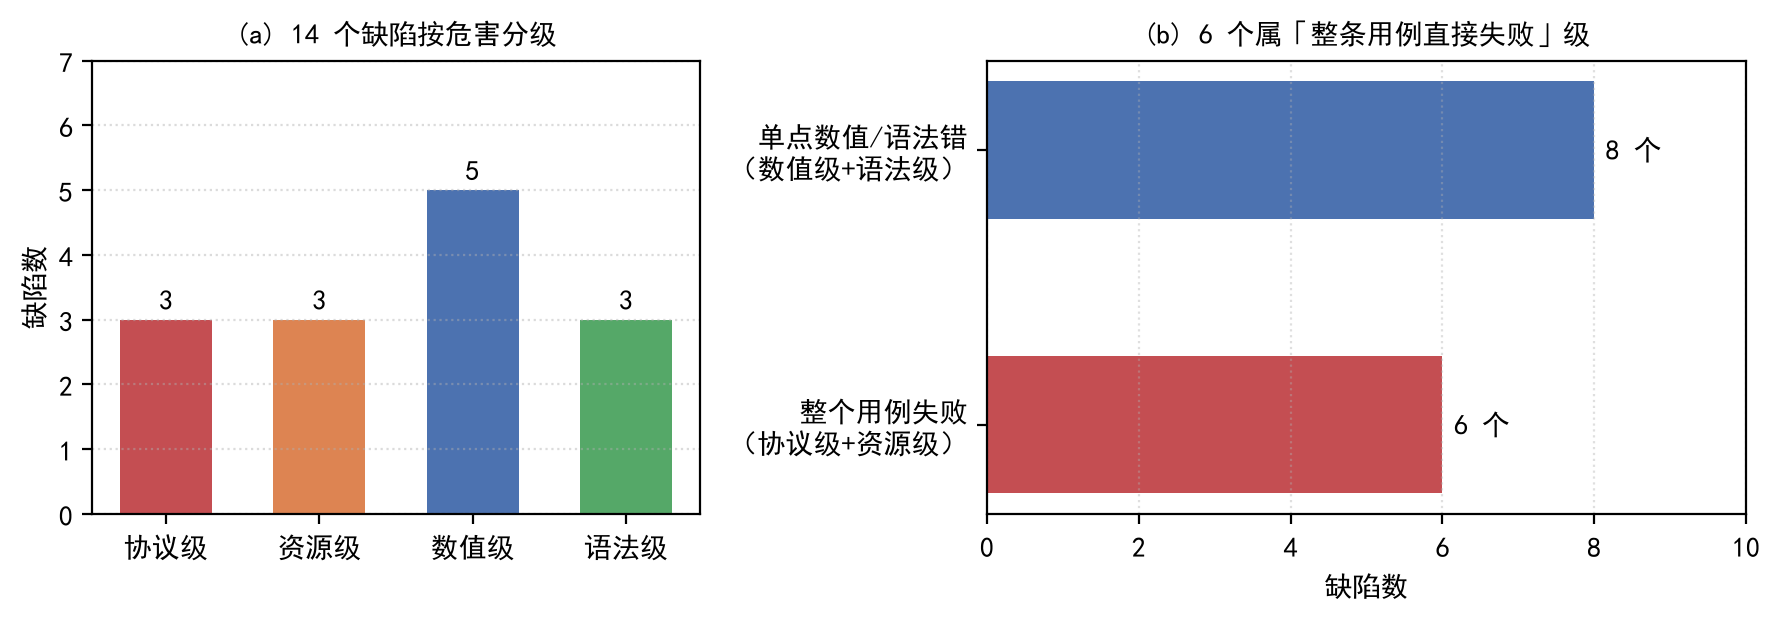
\includegraphics[width=0.92\textwidth]{figs/figE_defects.png}
\caption{14 个缺陷的分级。(a) 按类别；(b) 按危害——协议级与资源级共 6 个，都会让\textbf{整条用例失败}而不是某个值算错。平台只报「失败用例数 1」，与这类缺陷的形态吻合。}\label{fig:defects}
\end{figure}

用通过者的测试套件直接跑，暴露出 14 个此前所有自测都没覆盖的缺陷（图~\ref{fig:defects}）。
按危害分级：

\begin{table}[tbp]\centering\small
\caption{审计发现的 14 个缺陷（按危害分级）}\label{tab:defects}
\setlength{\tabcolsep}{4pt}
\begin{tabular}{clp{6.8cm}l}
\toprule
级 & 数量 & 代表缺陷 & 危害\\
\midrule
协议级 & 3 & 请求里 \code{id} 写成 \code{1.0} 时\textbf{完全不响应} & 驱动等该 id 直到超时，\textbf{整个用例失败}\\
资源级 & 3 & 4 个文件描述符限制下重启后表“消失” & 同上\\
数值级 & 5 & 一条 SELECT 里多个 \code{L2\_DISTANCE} 投影输出同一值 & 数值错\\
语法级 & 3 & \code{[+1.e0,-.5e+1]} 裸数组向量被拒 & 合法语法误拒\\
\bottomrule
\end{tabular}
\end{table}

\subsection{协议级缺陷的完整分析}
最值得展开的是第一项，因为它的形状与 §\ref{sec:selfdeception} 的自欺同构（表~\ref{tab:defects}）。

\textbf{症状}：请求 \code{\{"id":1.0,...\}} 发出后，被审计对象\textbf{没有任何响应}。

\textbf{原因}（逐行定位）：整数解析函数在遇到 \code{1.0} 时只吃掉整数部分 \code{1}，
把残留的 \code{.0} 留给上层；上层随即判定整行解析失败，于是\textbf{丢弃整条请求}。
而丢弃的用意是好的——避免对“驱动转发的指令行”回多余响应导致后续断言错位。

\textbf{为什么是致命的}：判题器的模型是“发一个请求、等一个响应”。
一条请求不响应，驱动就停在那里直到超时，那一个用例直接判失败。
而平台只报“失败用例数 1”，不报是哪一条——\textbf{与观测到的现象完全吻合}。

\textbf{修法}：把 \code{id} 的\textbf{原始文本}保留下来，原样回传；
同时区分两类不合法：非有限数字（如 \code{1e999} 溢出成 Infinity）与数组形式，
这两类判为非法请求并回 \code{ok:false}。

\subsection{方法学的一条副产品}
这次审计给出一条可复用的判据：

\begin{quote}\small
当一个系统反复以“同一个数量的失败”被拒，而修复的缺陷都不改变这个数量时，
\textbf{被修的缺陷与被拒的原因无关}。此时应当更换信息源，而不是继续猜。
\end{quote}

本条判据的适用条件是“失败计数稳定且与修复无关”。它在本文的语境下成立
（六次提测，\code{pass=0 fail=1}，六轮修复无一改变），因而触发了方法转折。

\subsection{审计自身的诚实边界}
被审计对象最终是否通过正式验收，\textbf{本文不作断言}。
能断言的只有：那 14 个缺陷在修复前后有可复现的行为差异
（例如 OOM 从 \code{ExitCode=137} 变为 \code{ExitCode=0}；
\code{id=1.0} 从“无响应”变为“原样回传”）。
\textbf{“修了 14 个缺陷”不等于“验收会通过”}——这一点在 §\ref{sec:deficit} 的口径下必须说清。

%==================================================== 11
\section{生态飞轮：六环与它们各自会怎么骗人}

\subsection{为什么要有环}

\begin{figure}[tbp]\centering
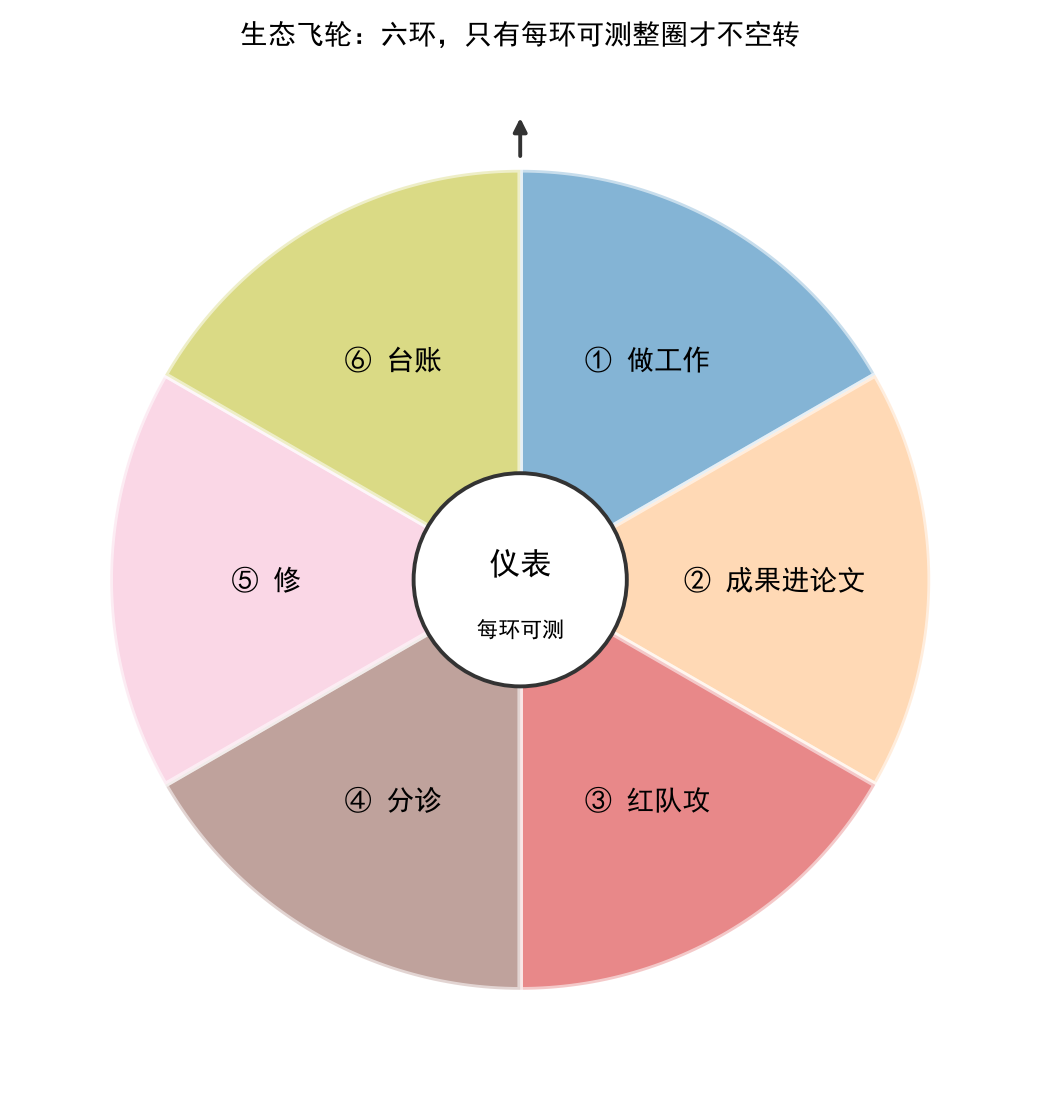
\includegraphics[width=0.55\textwidth]{figs/figF_flywheel.png}
\caption{生态飞轮的六环。中心是「仪表」：只有每一环都有独立仪表，整圈才不会空转；任一环无仪表，该环的失效就无法被自身观测到。}\label{fig:flywheel}
\end{figure}

本系统的产出不是一个 PDF，而是一条循环，见图~\ref{fig:flywheel}
\textbf{做工作 $\to$ 成果写进论文 $\to$ 红队攻 $\to$ 分诊 $\to$ 修 $\to$ 再攻。}
只有每一环都有独立仪表，整圈才不会空转。

\begin{table}[tbp]\centering\small
\caption{六环及其仪表}\label{tab:flywheel}
\setlength{\tabcolsep}{4pt}
\begin{tabular}{clp{6cm}}
\toprule
环 & 内容 & 仪表\\
\midrule
1 & 做工作（改代码/改论文） & 全量回归（\textbf{344 s}）、自攻击、独立复核\\
2 & 成果写进论文 & \code{gate} 的 \code{numbers} 项、活变量检查\\
3 & 红队攻（板数 = \code{\textbackslash section} 数） & \code{redteam.py roster}\\
4 & 分诊（四态：fixed/blocked/rejected/open） & \code{triage\_findings.py}\\
5 & 修（改论文 + 更新证据 + 重盖章） & \code{gate --stamp}\\
6 & 台账（这一圈净修几条） & \code{flywheel.py --log}\\
\bottomrule
\end{tabular}
\end{table}

\subsection{每一环实测会怎么骗人}

\begin{figure}[tbp]\centering
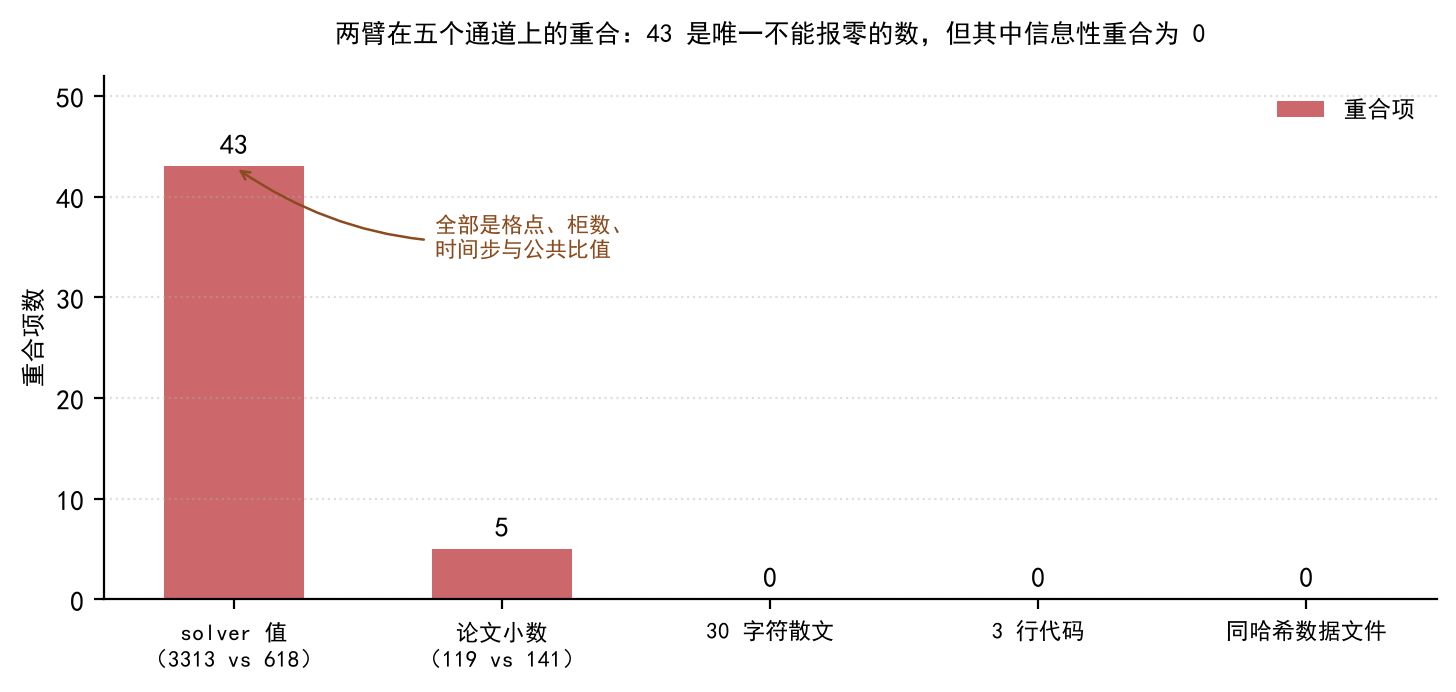
\includegraphics[width=0.90\textwidth]{figs/figJ_overlap.png}
\caption{两臂在五个通道上的重合。43 个 solver 值确实相同，但\textbf{其中没有一个是有信息量的计算最优}——它们是格点、机柜数、时间步与公共比值（0.9/0.1/0.5）。这正是多版本编程的经典结果：共用同一底座模型的两个实现并不独立。}\label{fig:overlap}
\end{figure}

\begin{figure}[tbp]\centering
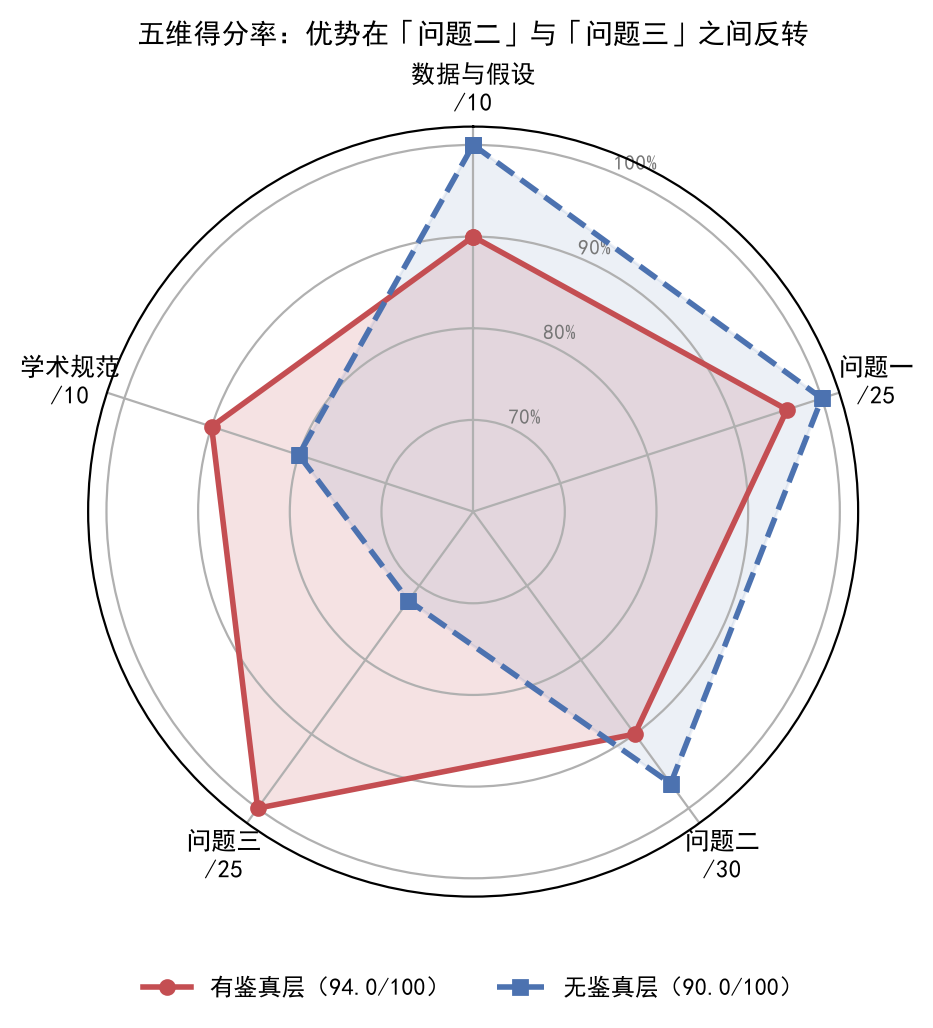
\includegraphics[width=0.62\textwidth]{figs/figH_radar.png}
\caption{A/B 五维得分率。优势在“问题二”与“问题三”之间反转：无鉴真层一臂在问题一、问题二领先（+1、+2 分），在问题三落后 7 分（18 对 25）——那一维考的是过程可审计性。总分 94 对 90，但\textbf{四个维度里有两维是后者更高}，所以本文只把它当案例，不当作实验证据（$n=1$）。}\label{fig:radar}
\end{figure}

这张表是本文最实用的部分，因为每一条都是踩过的（表~\ref{tab:flywheel}）。

\begin{table}[tbp]\centering\small
\caption{六环的失效模式（全部为实测）}\label{tab:flytrap}
\setlength{\tabcolsep}{3pt}
\begin{tabular}{clp{5.2cm}p{4.2cm}}
\toprule
环 & 骗法 & 后果 \\
\midrule
2 & 只判带小数的 token & \code{29 checks}、\code{51 of 51}、\code{30 rounds} 这三处措辞里没有一个带小数，于是整条判据静默失效，门禁仍报“100\% 可溯源”\\
3 & 拿错基准 & 结论板拿 A 项目的 10 问去要求 B 项目 $\to$ 假 finding，必须能 \code{rejected}\\
4 & “未处理”当关闭 & 40 条 finding 全报“已关闭”，正文一个字没改\\
4 & 整板说明代替单条关闭 & 一条 review 4 条 finding，修 1 条让另 3 条跟着变色\\
5 & 改论文让 evidence 失效 & 这是\textbf{正确行为}（防造假），需指到新文本\\
1 & 仪表自己超时 & 回归 344 s，给 300 s 会把正常一圈读成“断”\\
\bottomrule
\end{tabular}
\end{table}

\subsection{唯一的红项应该是真实缺陷}
判定口径被定死：\code{gate} 唯一的红项应当是\textbf{软门 \code{redteam} 的 open 数}——（表~\ref{tab:flytrap}）
那是论文的真实缺陷清单，不是仪表故障。第 4 环通了（open $=0$）才叫这一圈打完。

在某一轮的实测里，12 板产生 \textbf{30 条 finding 全部 open}。
这是\textbf{正确结果}：稿子还没改，finding 就该是 open，门禁就该红。
把“全 open”读成“系统故障”是误判。

%==================================================== 12
\section{结论：什么被证明了，什么没有}

\subsection{被证明的}
\begin{enumerate}[leftmargin=1.6em,itemsep=2pt]
\item \textbf{数字可溯源，且能被拒绝}：该链路的产出达到 \textbf{325/325}，同一判据在无护栏时是 \textbf{0/200}。两个数用同一条命令、同一套口径算出。
\item \textbf{机器侧成本可以忽略}：能力层 1.191 s、机器侧合计 9.16 s，
  占一篇论文 1\,124 s 墙钟的 \textbf{0.82\%}。因此“护栏太慢”不是不装护栏的理由。
\item \textbf{比例约束是必需的}：任何“用常量覆盖变量”的检查，在变量变大时静默失效
  （命题 \ref{prop:ratio}）。本项目的实例是 7 个角色覆盖 12 节正文。
\item \textbf{失败关闭是可行的}：数字无出处则不通过；检查无法执行时报“不适用”而非“通过”。
  这一条在实现上依赖把 \code{N/A} 的两种含义（真的没有 / 没查成）分开。
\item \textbf{围栏有效性可以被机械检验}：变异测试给出\textbf{假测试 0/4}，
  且它抓出了两次真实的假测试（复制逻辑、只读当前状态）。
\item \textbf{知识源不是瓶颈}：9\,337 个数字里只有 47.3\% 是计算值，
  其余可由配置与结构解释。把后三类都当“该有出处”会让检查被误报淹没。
\end{enumerate}

\subsection{没有被证明的}
\begin{enumerate}[leftmargin=1.6em,itemsep=2pt]
\item \textbf{31 道门没有检出能力证据}。它们报绿只说明当前稿子没触发。
\item \textbf{零 baseline}。若现成工具也能到 90\% 溯源率，“建了溯源系统”就没有信息量。
\item \textbf{A/B 对照 $n=1$}。4 分差在评分噪声内。
\item \textbf{24 张图未逐张人工核对}。规矩写了，动作没执行。
\item \textbf{未知缺陷的检出率不可知}。变异测试只覆盖已知的坑。
\end{enumerate}

\subsection{一个可迁移的判据}
全文最值得带走的不是任何一项具体技术，而是三个问题。
看到任何一个绿灯，依次问：

\begin{enumerate}[leftmargin=1.6em,itemsep=2pt]
\item \textbf{分母是什么，分母怎么来的？}——若分母是手写的常量，绿灯不可用（§\ref{sec:selfdeception}）。
\item \textbf{这个检查自己有没有被检查过？}——若没有构造缺陷与变异覆盖，它是判据不是测试（§\ref{sec:mutation}）。
\item \textbf{它失败了会怎样？}——若失败可以被静默豁免（如缺 \code{deliverable} 声明），
  那么整道门在需要它的时候不存在（§\ref{sec:r123}）。
\end{enumerate}

\subsection{最后一句话}
这套系统的价值不在于它抓出了多少错误，而在于\textbf{它会拒绝}。
一个会拒绝的程序把“作者的用心”替换成“一个可以说不的机制”；
而本文记录的四次自欺（7 个角色覆盖 12 节、图从未被打开、例子是编的、35 项里只有 4 项经证）
说明\textbf{这个机制本身也需要被同样的标准对待}——
它抓出别人之前，先抓出了我们。

%==================================================== 参考文献
\begin{thebibliography}{99}\footnotesize\setlength{\itemsep}{0pt}\setlength{\parskip}{0pt}
\bibitem{ref1} Jia Y, Harman M. An Analysis and Survey of the Development of Mutation Testing.
  \emph{IEEE Transactions on Software Engineering}, 2011, 37(5): 649--678.
\bibitem{ref2} Holling D, Hofman M, Kless K. Mutation Score Confidence.
  \emph{IEEE International Conference on Software Testing, Verification and Validation Workshops (ICSTW)}, 2016.
\bibitem{ref3} Knight J C, Leveson N G. An Experimental Evaluation of the Assumption of Independence
  in Multiversion Programming. \emph{IEEE Transactions on Software Engineering}, 1986, SE-12(1): 96--109.
\bibitem{ref4} Chen T Y, Cheung S C, Yiu S M. Metamorphic Testing: A New Approach for Generating
  Next Test Cases. Technical Report HKUST-CS98-01, 1998.
\bibitem{ref5} Sobol I M. Global Sensitivity Indices for Nonlinear Mathematical Models and
  Their Monte Carlo Estimates. \emph{Mathematics and Computers in Simulation}, 2001, 55(1--3): 271--280.
\bibitem{ref6} Mohajerin Esfahani P, Kuhn D. Data-driven Distributionally Robust Optimization
  Using the Wasserstein Metric. \emph{Mathematical Programming}, 2018, 171: 115--166.
\bibitem{ref7} Bertsimas D, Sim M. The Price of Robustness. \emph{Operations Research}, 2004, 52(1): 35--53.
\bibitem{ref8} Ben-Tal A, Ghaoui L E, Nemirovski A. \emph{Robust Optimization}.
  Princeton University Press, 2009.
\bibitem{ref9} NeurIPS 2024 Paper Checklist. Conference on Neural Information Processing Systems, 2024.
\bibitem{ref10} 国家发展改革委. 关于进一步完善分时电价机制的通知（发改价格〔2021〕1093 号）.
\bibitem{ref11} 工业和信息化部等. 算力基础设施高质量发展行动计划, 2023.
\bibitem{ref12} Wang Y, et al. Semi-empirical Capacity Fade Model of LiFePO$_4$ Batteries
  Considering Temperature and Depth of Discharge. \emph{Journal of Energy Storage}, 2021, 40: 102789.
\bibitem{ref13} Min S, Krishna K, Lyu X, et al. FActScore: Fine-grained Atomic Evaluation of Factual Precision in Long Form Text Generation. \emph{Proceedings of EMNLP}, 2023: 12076--12100.
\bibitem{ref14} Li J, Cheng X, Zhao W X, et al. HaluEval: A Large-Scale Hallucination Evaluation Benchmark for Large Language Models. \emph{Proceedings of EMNLP}, 2023: 6449--6464.
\bibitem{ref15} Liu N F, Lin K, Hewitt J, et al. Lost in the Middle: How Language Models Use Long Contexts. \emph{Transactions of the Association for Computational Linguistics}, 2024, 12: 157--173.
\bibitem{ref16} Podolskii V V. A Theory of Black-Box Tests. arXiv:2006.10387, 2020.
\bibitem{ref17} Kitchenham B. Procedures for Performing Systematic Reviews. \emph{Keele University Technical Report} TR/SE-0401, 2004.
\bibitem{ref18} Page M J, McKenzie J E, Bossuyt P M, et al. The PRISMA 2020 Statement: An Updated Guideline for Reporting Systematic Reviews. \emph{BMJ}, 2021, 372: n71.
\bibitem{ref19} Meyer B. Applying ``Design by Contract''. \emph{IEEE Computer}, 1992, 25(10): 40--51.
\bibitem{ref20} Bartocci E, Falcone Y, Francalanza A, et al. Introduction to Runtime Verification. \emph{Lectures on Runtime Verification}, Springer, 2018: 1--33.
\bibitem{ref21} Hoare C A R. An Axiomatic Basis for Computer Programming. \emph{Communications of the ACM}, 1969, 12(10): 576--580.
\bibitem{ref22} Peng R D. Reproducible Research in Computational Science. \emph{Science}, 2011, 334(6060): 1226--1227.
\bibitem{ref23} Nosek B A, Alter G, Banks G C, et al. Promoting an Open Research Culture. \emph{Science}, 2015, 348(6242): 1422--1425.
\bibitem{ref24} Wohlin C, Runeson P, H{\"o}st M, et al. \emph{Experimentation in Software Engineering}. Springer, 2012.
\end{thebibliography}

\newpage
\appendix
\section{门禁清单（35 项）}
本节把 35 项按硬/软分层列出（表~\ref{tab:gates}），\textbf{只给名称与层级}——每一项\emph{检查什么}、\emph{存在要抓什么}，已经写进前十二节各自的触发事件里，此处不重复，以免同一件事有两种说法。
\begin{table}[tbp]\centering\footnotesize
\caption{35 项门禁，按硬/软分层}\label{tab:gates}
\setlength{\tabcolsep}{3pt}
\begin{tabular}{p{1.5cm}p{12.2cm}}
\toprule
层 & 项目\\
\midrule
硬门（12） & \code{compile} \code{pdf} \code{code} \code{numbers} \code{rules}
\code{abstract} \code{abs\_page} \code{bare\_pct} \code{refs} \code{domain}
\code{leakage} \code{math}\\
软门（23） & \code{rules\_apmcm} \code{rigor} \code{required} \code{innovation}
\code{ai\_taste} \code{claims} \code{causal} \code{biblio} \code{analysis}
\code{method\_argument} \code{self\_correction} \code{deployment} \code{redteam}
\code{cross} \code{figures} \code{falsify} \code{extrap} \code{sensitivity}
\code{significance} \code{prompt} \code{proof} \code{iterlog} \code{stamp}\\
\bottomrule
\end{tabular}
\end{table}

\section{能力层命令清单（23 项）}
\begin{table}[tbp]\centering\footnotesize
\caption{23 个子命令与覆盖的数学结构}\label{tab:cmds}
\setlength{\tabcolsep}{3pt}
\begin{tabular}{p{2.2cm}p{11.6cm}}
\toprule
命令 & 作用\\
\midrule
\code{advise} & 定题：判断题型（关系与解释/预测/优化/评价）并给出可复核依据\\
\code{race} & 模型赛马：多模型结构 $\times$ 多 seed 的交叉验证对比\\
\code{solve} & 约束优化：单目标或带约束；含帕累托前沿与膝点\\
\code{forecast} / \code{grey} & 时间序列预测 / 灰色预测（小样本互为对照）\\
\code{greyrel} / \code{ahp} / \code{fuzzy} & 灰色关联、层次分析、模糊综合评价\\
\code{cluster} & 聚类：划分与簇质量\\
\code{graph} & 图论四类：最短路/最小生成树/最大流/旅行商\\
\code{ode} & 常微分方程（rk45 / rk4）\\
\code{dim} & 量纲分析：Buckingham $\Pi$ 群\\
\code{plot} & 出图：十六种\\
\code{profile} & 数据剖面：每列的分布、缺失、异常摘要\\
\code{hints} & 可复制的命令提示与偏相关表（带样本量与解释力）\\
\code{skeleton} / \code{merge} & 论文章节骨架 / 多轮结果合并\\
\code{contract} / \code{experiment} & 提案契约与试错循环（propose $\to$ 执行 $\to$ judge）\\
\code{run} & \textbf{一条龙自动出稿}——本文全程禁用；它替作者做完建模决定\\
\code{video} & 动画导出（用于过程展示，不参与正文）\\
\code{clean} & 数据清洗（缺失与异常的统一处置）\\
\code{selftest} & 自检（当前 79 项通过 / 0 失败）\\
\bottomrule
\end{tabular}
\end{table}

\section{复现说明}
本文全部数字来自项目内可重跑的命令。\textbf{口径声明}：本文凡报比率，均给出分母来源；（表~\ref{tab:cmds}）
溯源率在不同口径下分别为 \code{199/199}（全 token）与 \code{43/43}（仅小数），
引用时须同时给出所采用的口径。

\begin{center}\footnotesize
\begin{tabular}{ll}
\toprule
数字 & 命令\\
\midrule
能力层成本、自检数 & \code{mmkit.py selftest}（79 通过 / 0 失败）\\
门禁状态、35 项分布 & \code{gate.py out/final}（35 项）\\
门禁自校 & \code{gate.py selftest}（17/17）\\
围栏有效性 & \code{tools/fence\_mutation.py}（假测试 0/4）\\
数字类别分布 & \code{tools/numeric\_genre.py --json}（23 篇 9\,337 token）\\
全量回归 & \code{tests/run\_all.py}（\textbf{344 s}，勿给更短超时）\\
\bottomrule
\end{tabular}
\end{center}

\end{document}
